\documentclass[runningheads]{llncs}
%
\usepackage{graphicx}

\usepackage{natbib}
\setcitestyle{square,numbers}

\usepackage[toc,page]{appendix}

\usepackage{nameref}

% \usepackage{amsthm}
\usepackage{amsmath}
\usepackage{amssymb}
\usepackage[ruled,vlined]{algorithm2e}

\usepackage{xcolor}
\usepackage{pdfpages}

\def\HiLi{\leavevmode\rlap{\hbox to \hsize{\color{yellow!50}\leaders\hrule height .8\baselineskip depth .5ex\hfill}}}
         
\newcount\Comments  % 0 suppresses notes to selves in text
\Comments=0
\definecolor{darkgreen}{rgb}{0,0.6,0}         
         
\newcommand{\kibitz}[2]{\ifnum\Comments=1{\color{#1}{#2}}\fi}
\newcommand{\rmr}[1]{\kibitz{red}{[Reshef says:#1]}}
\newcommand{\rf}[1]{\kibitz{blue}{[Roy says:#1]}}
\newcommand{\kg}[1]{\kibitz{darkgreen}{[Kobi says:#1]}}

\begin{document}

%
\title{Proportional Participatory Budgeting with Substitute Projects}
%
%\titlerunning{Abbreviated paper title}
% If the paper title is too long for the running head, you can set
% an abbreviated paper title here
%

\author{Submission 16}
% \author{Roy Fairstein\inst{1}\orcidID{0000-0002-2352-5200} \and
% Reshef Meir\inst{2}\orcidID{0000-0003-0961-3965} \and
% Kobi Gal\inst{1,3}\orcidID{0000-0001-7187-8572}}
%
\authorrunning{Submission 16}
\institute{}
% \authorrunning{Fairstein et al.}
% First names are abbreviated in the running head.
% If there are more than two authors, 'et al.' is used.
%
% \institute{Ben-Gurion Univ. of the Negev, Israel \and
% Technion, Israel Institute of Technology \and
% Ben-Gurion Univ. of the Negev, Israel, University of Edinburgh, U.K.}
%
\maketitle              % typeset the header of the contribution
%
\begin{abstract}
Participatory budgeting is a democratic process for allocating funds to projects based on the votes of members of the community. \rmr{removed: The goal is to fund the projects   which are best for the community, according to voters' preferences.} In many cases, voters preferences over projects are complex, most input methods of voters' preferences  prevent the voters from expressing dependencies among projects, leading to outcomes that do not reflect their preferences well enough. In this paper, we propose an  input method that allows participants to express substitutes over projects.  We  extend a  mechanism based on Rule~X (\citet{peters2020proportional})  input with substitutes, and show that the extended rule preserves proportionality under some constraints. We show in simulations that the extended rule obtains  substantially more welfare than the original Rule~X.

\keywords{Participatory Budgeting, Social Choice, Fairness}
\end{abstract}
%
%
%
\section{Introduction}

%The first Participatory budgeting project had started a while back in Brazil in the 1980s \cite{cabannes2004participatory}, with the goal of creating a more transparent funding process and giving more power to citizens. Since then, 
Participatory budgeting is gaining increased attention and is now in use in many places such as  Cambridge, Chicago, New York and Paris~\cite{pape2016budgeting, su2017porto, sintomer2008porto}. 
%In participatory budgeting  citizens decide how to allocate some common budget in order to fund projects that will increase their life quality. The 
This process typically includes several steps: first, the citizens are able to suggest and discuss  different ideas, resulting with a   list of feasible ideas and  their cost estimation. Next,  the citizens vote on which of the projects they would like to be fund. Finally, the votes are aggregated by a mechanism which outputs the   projects to be funded.






There are many ways for voters to express their preferences over the different   projects (different input formats), such as approval, knapsack ranking and additive utility \cite{aziz2020participatory,goel2016knapsack,aziz2020expanding, benade2020preference,peters2020proportional}. 
In the real world, the preferences of a voter over projects may be dependent, i.e., the utility from one project might depend on whether some other project is funded or not \cite{jain2020participatory}.

Consider for example a city where there are 4 different suggestions to build a large parking lot in different places in a district, as well as two unrelated projects (say, a playground and a library). The budget is sufficient for only four projects.
There is a severe parking problem, so most citizens will assign higher utility to parking lots than to the other projects (or rank parking lots higher in a ranking-based platform). As a result all 4 parking lots are likely to be funded and consume the entire budget, even if one or two parking lots are sufficient to solve most of the parking shortage.
A better outcome that leads to a higher social welfare would have been to fund only two parking lots, and in addition the playground and the library. 
The above problem occurs since most existing mechanisms ignore the fact that the four parking lots are \emph{substitutes}. Indeed, additive cardinal utilities or rankings cannot convey such relations. 

In this paper,  we suggest an input format and aggregation mechanism which allow  voters to express substitute relationships and output socially beneficial outcomes.
 Our input format  allows  the voters to declare groups of substitute projects and   a diminishing marginal utility function for each group. 
Our  voter from the previous example could declare all parking lots as substitutes, and specify a high utility for the first parking lot that is selected, some lower utility for the second parking lot that is  selected, and zero marginal utility for the third and fourth parking lots. 

In the second stage, after all voters have voted, we want to aggregate their votes and select which projects to fund.
Two common ways to measure quality of this outcome  is by social welfare and proportionality  (having all parts of the population well represented).
%The term "proportionality" can be understood in different ways, and we will present several commonly used definitions from the literature.
%So what makes a given outcome a ``good" outcome? There are different ways to answer this question.
% 
There is an inherent tradeoff between proportionality and social welfare: Consider our running example above with budget that is only sufficient for two projects, where only 45\% of the voters own a car (so they care about parking), while the others only want the playground and the library. Selecting the library and the playground would maximize social welfare, but leaves almost half of the population without any desired project. A more fair (proportional) solution would be to fund one of the parking lots along with one of the other projects. 
 Our suggested mechanism  improves the social welfare using the substitutes information while keeping the outcome  proportional.


The main contributions of this work are: (1) we suggest a simple way for the voters to  express preferences with substitutes; (2) We extend an existing aggregation mechanism called Rule~X~\cite{peters2020proportional} to support such preferences; (3) We prove the modified mechanism is proportional under certain assumptions on the input; (4) We show using simulations, that the new mechanism achieves outcomes with better social welfare compared to Rule~X while being also proportional.


%%%%%%%%%%%%%%%%%%%%%%%%%%%%%%%%%%%%%%%%%%%%%%%%%%%%%%%%%%%%%%%%%%%%%%%%

\subsection{Related Work}
The participatory budgeting literature defines and studies various notions of proportionality~\cite{peters2020proportional, fain2016core, fain2018fair, aziz2017proportionally, aziz2017justified, sanchez2016proportional, skowron2020participatory}. We formally define and discuss some of these notions in Section~\ref{sec:prop}.

Other papers focus on social welfare, such as  ~\citet{goel2019knapsack} which shows that when using the  knapsack input format  it is possible to achieve an outcome that maximizes the social welfare.
 \citet{jain2020participatory} considers special cases where it is possible to find a polynomial time algorithm which maximizes the social welfare. 
The tradeoff of welfare and proportionality is studied in \cite{michorzewski2020price}. %shows the price of fairness, i.e. the price the social welfare ``pays" for requiring the outcome to be fair. 
This tradeoff has also been studied in the context of multi-winner elections~\cite{skowron2018proportionality, lackner2020utilitarian} (which are participatory budgeting with unit cost for projects).
%such as  which shows proportionality and welfare guarantees different mechanism can achieve. Those results also show the trade-off between the two.

The literature suggests many different ways to 
represent voter preferences over a discrete set of projects, such as approval voting \cite{aziz2020participatory, aziz2017proportionally}, knapsack voting \cite{goel2019knapsack, goel2016knapsack, fluschnik2019fair}, ranking \cite{aziz2020expanding, benade2020preference} and reporting utilities \cite{peters2020proportional} for each of the projects. However, all of those methods ignore substitution among projects. %the fact that can projects can have some effect on each other for some voter. One such connection is substitution between project.
One exception is \citet{jain2020participatory} who tackle the issue of substitute projects. They suggest a way to describe  interactions between projects using approval voting, while allowing 
projects to be  substitutes  or complimentary to each other. 
They suggest a mechanism for finding set of  projects for special cases which  optimize social welfare in polynomial time, disregarding the notion of proportionality. In contrast, our mechanism, while 
also polynomial in all cases,    improves the social welfare while keeping the outcome proportional. %Another difference is that \citet{jain2020participatory} assumes the project groups are pre-defined while our method allows voters to define them.

 \citet{peters2020proportional}  present a new aggregation rule for participatory budgeting called Rule~X which can handle cardinal utilities and results with an outcome which is proportional.  We  extend this mechanism to support substitute projects.
 
Finally, while  this paper focus on participatory budgeting with indivisible projects, there is an area in participatory budgeting when the projects are divisible, i.e. it is possible to fund only parts of the project. In this area, there are a bit more optimistic results, Fain et al.~\cite{fain2018fair} succeed in designing an algorithm to calculate outcome which are in the core (the strongest definition currently used to describe proportionality in participatory budgeting) for a broad class of utility functions.


%%%%%%%%%%%%%%%%%%%%%%%%%%%%%%%%%%%%%%%%%%%%%%%%%%%%%%%%%%%%%%%%%%%%%%%%

\section{Preliminaries}
We denote for $a\in \mathbb{N}$,  $[a]:=\{1,\ldots,a\}$.
We define the Participatory budgeting (PB) instance as an election tuple $(V,A,cost,L)$, where:
\begin{enumerate}
    \item $N=[n]$ is a set of n voters participating in this election.
    \item $A=\{a_1,\ldots,a_M\}$ is a set of M alternatives (projects) which are considered in the election.
    \item cost: $A\rightarrow \mathbb{R}_+$ is a function specifying the cost of each project $p\in A$. The cost for subset of alternatives $T\subseteq A$ is $cost(T)=\sum_{p\in T}cost(p)$.
    \item $L\in \mathbb{R}_+$ is the total budget the voters have in order to fund the selected alternatives. 
\end{enumerate}
 
 For some voter $i\in V$, we define $A(i)$ is the set of projects that voter $i$ approves. While this notation fits approval based rules, we will use A(i) also for other rules to denote all projects where the utility for voter i is more than 0.
     For each voter $i\in V$ and bundle of projects $B\subseteq A$, $u_i(B)$ represents the utility that voter i get for bundle B. for a group of voters $S\subseteq V$ it can be extended: 
$$u_S(B)=\sum_{i\in S}u_i(B).$$
 The purpose of PB instance is to choose some bundle $B\subseteq A$ of projects which is feasible, i.e. $cost(B)\leq L$. 


%%%%%%%%%%%%%%%%%%%%%%%%%%%%%%%%%%%%%%%%%%%%%%%%%%%%%%%%%%%%%%%%%%%%%%%%

\section{Preference Modeling}\label{input}


Throughout the paper we will assume that the preferences expressed by voters are their real preferences.  
The most expressive way to represent the voters' preferences is using a utility function $U_i:2^A\rightarrow \mathbb R$  for each voter $i\in V$,  i.e. for each feasible bundle $B\subseteq A$, $U_i(B)$ is the utility that voter~$i$ gives bundle~$B$. While this option enables us to express all possible preferences, expressing the utility for every feasible bundle can be very tiresome and inaccurate.
% how does one request from a voter to express his utility for every feasible bundle (with exponential amount of options)? A task which is very tiresome, and even if a voter succeeds with it, it might not be very accurate. 

On the other extreme we can represent whether voters approve each project (approval voting), 
which is far less expressive. 
Because this representation is the simplest, it is the most common representation used \cite{aziz2020participatory, aziz2017proportionally}.
%In approval voting, each voter can choose for each project whether they want it to be funded or they don't want it to be funded, i.e. additive utilities where utilities can only be 0 or 1. 
Usually in the context of participatory budgeting, $k$-approval is used, where the voters are limited to approving $k$ projects.

Between those two extreme ways of representing the voters preferences, there are several 
representations which vary in their expressiveness. The first one,   similar to $k$-approval, is knapsack \cite{goel2019knapsack, goel2016knapsack, fluschnik2019fair}, where voters are  limited to a given budget, rather than the number of projects. Another option is asking the voters to rank the projects from the one they want the most to the one they want the least \cite{aziz2020expanding, benade2020preference}. Lastly, voters are requested to assign a utility to each project \cite{peters2020proportional}.


None of the representations above allows for dependencies among projects. To address this challenge, we allow voters to express substitute relationships over projects. Specifically, we let  each voter $i\in [n]$ split the projects into $k_i$ groups $v_i=\{g_1,\ldots,g_{k_i}\}$ (each voter can have different amount of groups), where $\cup_{g\in v_i}g\subseteq A$ and $\forall k_1\neq k_2 \in \{1,\ldots,k_i\}, g_{k_1}\cap g_{k_2}=\emptyset$.
 We denote by $g_i(a)$ the set of projects that $i$ considers as substitutes for $a$.
For each of those groups, the voter holds a marginal utility function $u_{ig}:[M]\rightarrow \mathbb{R}_+$, which represents the marginal utility voter $i$ receive for funding the $j$'th project in $g$. The utility of projects from different groups is additive, thus 

\vspace{-3mm}
$$u_i(B):=\sum_{g\in{v_i}}\sum_{j=1}^{|g\cap B|}u_{ig}(j).$$
 
 The above formalism does not constrain the shape of the utility function, but we focus only on non-increasing marginal utility functions, in order to capture substitutes.
In addition, we require that $\forall i\in V, \forall g\in v_i,$ the utility $u_{ig}(1)=I$ where $I$ is a constant (or equal to 0 if the voter does not want any of the projects in $g$). That is, first project in each group of substitutes has the same utility, as in approval voting. 

we provide a few examples for  marginal utility functions:
\begin{enumerate}
    \item Unit demand: This is the strongest case of substitute projects, where the voter does not benefit at all from substitute projects. The voter wants exactly one project from each substitute group, formally: $$\forall i\in V, \forall g\in v_i, u_{ig}(k)= 
        \begin{cases}
            I             ,& \text{if } k=1\\
            0,             & \text{otherwise}
        \end{cases}$$
    Resulting with voter utility for bundle $B\subseteq A$: $$u_i(B)=I\cdot|\{g : g\in v_i, |g\cap B|>0\}|.$$

    \item Minimal substitutes: This utility specifies that the voter strongly prefer projects that are not substitutes.  The voter prefers  a project with no substitute projects funded over funding $|A|$ projects that are substitutes.
    % The voter strictly prefers one project where none of its substitute projects were funded over a project which is substitute to some project that was funded. 
    This is done by giving a utility of $I$ for the first project in each group, and utility of $\frac{I}{|A|}$ for any addition project in the same group. Formally: $$\forall i\in V, \forall g\in v_i, u_{ig}(k)= 
        \begin{cases}
            I                         ,& \text{if } k=1\\
            \frac{I}{|A|},             & \text{otherwise}
        \end{cases}$$
    This means that adding a single project from a new group is worth to the voter more than adding all substitutes of selected projects.
    
    \item PAV based utility \cite{thiele1895om}:  The marginal utility for each substitute group is the reciprocal function. Formally: $\forall i\in V, \forall g\in v_i, u_{ig}(k)=\frac{I}{k}$. The voter's utility is then a sum of harmonic series: $$u_i(B)=\sum_{g\in{v_i}}\sum_{k=0}^{|g\cap B|}\frac{I}{k}.$$
\end{enumerate}


%%%%%%%%%%%%%%%%%%%%%%%%%%%%%%%%%%%%%%%%%%%%%%%%%%%%%%%%%%%%%%%%%%%%%%%%

\section{Aggregating Votes}
Thus far, we described a way for voters to express their preferences by letting them report groups of substitute projects. The next stage after receiving those votes, is to aggregate the votes in order to choose a bundle of projects to fund. To do so, we need a new aggregation method that will take into account the fact that there are substitute projects.


Our starting point is the Rule~X (RX) algorithm recently introduced by \citet{peters2020proportional}. 
%Since RX was defined for additive utilities, we modify it to  deal with substitute utilities in the format we defined above called Substitute Rule X (SRX). 
%We begin by stating the  definition of RX, following with our extension to support substitute projects.
%Rule X (RX) - 
RX is an iterative rule, which starts with ``allocating" each voter an equal share of the budget $\frac{L}{|V|}$, and  initialize an empty outcome $B=\varnothing$; then sequentially adds projects to $B$. At each step, in order to choose some project $p\in A\setminus B$, each voter needs to pay an amount that is proportional to her utility from the project, but no more than her remaining budget (note that with approval utilities this means only agents that approve the project pay). The  total payment should cover the cost of the project. 
 
 Formally, let $b_i(t)$ be the amount of money that voter~$i$ is left with just before iteration~$t$.
 We say that some project $p\in A$, is $q$-affordable if $\exists q\in \mathbb{R}_+$ such that 
$$\sum_{i\in V}min(b_i(t),U_i(p)\cdot q)\geq cost(p)$$
Where $U_i(p)$ is the utility of voter $i$ for project $p$.

If no candidate project is q-affordable for any $q$, Rule~X terminates and returns $B$. Otherwise it selects project $p^{(t)}\notin B$ that is $q$-affordable for a minimum $q$, where individual payments are given by $c_i(p^{(t)}):=\min\{b_i(t),u_i(p^{(t)})\cdot q\}$. Then we update the remaining budget as $b_i(t+1):=b_i(t)-c_i(p^{(t)})$.

 The pseudocode for calculating the  qValue for a given project is shown in Algorithm~\ref{algo:qval}.  
The pseudocode for RX is given in Algorithm~\ref{algo:srx} (without the highlighted line).

\begin{algorithm}[t]
\SetAlgoLined
\textbf{Input:} 
\begin{enumerate}
    \item project $p\in A$ \\ 
    \item $\forall i\in V,  U_i(p)$ \rmr{what is $S$?}\rf{fixed}\\
    
\end{enumerate}
\KwResult{q-value computation for project $p$}
\If {$\sum_{i\in v, U_i(p)>0}b_i(t)< cost(p)$}
 {$return \  \infty$}
 
 $current\_utility \leftarrow \sum_{i\in V}U_i(p)$
 
 $cost\_leftover \leftarrow cost(p)$
 
 $removed\_voters \leftarrow \varnothing$
 
 \While{True}{
    $current\_q \leftarrow cost\_leftover /    current\_utility$
    
    $voter\_removed \leftarrow False$
    
    \For{$i\in V\setminus removed\_voters$}{
      \If{$current\_q * U_i(p) > b_i(t)$}{
            $current\_utility \leftarrow current\_utility - U_i(p)$
            
            $cost\_leftover \leftarrow cost\_leftover - b_i(t)$
            
            $removed\_voters \leftarrow removed\_voters \cup \{i\}$
            
            $voter\_removed \leftarrow True$
       }
       
     }
     
     \If{$voter\_removed == False$}{
            $return \  (cost\_leftover / current\_utility)$
       }
 }

 \caption{qValue}\label{algo:qval}
\end{algorithm}

% \begin{algorithm}
% \SetAlgoLined
% \textbf{Input:}
% \begin{enumerate}
%     % \item $\forall i\in S, \forall g\in v_i,  u_{ig}$ \\
%     \item $\forall i\in S, \forall p\in A, U_i(p)$
%     \item Budget given L \\
%     \item $\forall p\in A, cost(p)$
% \end{enumerate}

% \KwResult{Feasible bundle $B\subseteq A$}
%  $B_0 \leftarrow \varnothing$
 
%  $t \leftarrow 0$
 
%  $\forall i\in S: b_i(t) \leftarrow\frac{L}{|V|}$
 
%  \While{True}{
%   $chosen\_project \leftarrow argmin_{p\in A\setminus B_t}[qValue(p, U_{[|A|]})]$
  
%   \If{$qValue(chosen\_project)=\infty$}{
%         $return \  B_t$
%   }
%   $B_{t+1} \leftarrow B_t \cup \{chosen\_project\}$
   
%   $\forall i\in S: b_i(t) \leftarrow b_i(t) - min(b_i(t),U_i(chosen\_project)\cdot q)$
   
%   $t \leftarrow t + 1$
%   }
%  \caption{Rule X aggregation}\label{algo:rx}
% \end{algorithm}


One drawback of RX is that it assumes additive utilities and does not take into account  project substitutes (recall the parking lots example from the introduction).
%where one parking lot is enough for a voter, but he doesn't have a way to express it, so he might approve all of them to increase the chance of getting one of them funded, causing more then one to be funded.
In order to handle this issue, we will now extend RX to Substitute Rule X (SRX) which takes into account substitute projects. This is by updating the \emph{marginal} value of each project after every iteration.



\begin{algorithm}
\SetAlgoLined
\textbf{Input:}
\begin{enumerate}
    \item $\forall i\in V, \forall g\in v_i, \forall p\in A,  u_{ig}(p)$ \rmr{either $\forall i\in V, \forall g\in v_i,   u_{ig}$ or $\forall i\in V, \forall g\in v_i, \forall p\in A,  u_{ig}(p)$}  \\
    \item Budget $L$ \\
    \item $\forall p\in A, cost(p)$
\end{enumerate}

\KwResult{Feasible bundle $B\subseteq A$}
 $B_0 \leftarrow \varnothing$
 
 
 $\forall i\in V: b_i(0) \leftarrow\frac{L}{|V|}$ \rmr{what is $S$? you mean $V$?}\rf{fixed}
  $t \leftarrow 1$

 \While{True}{
    \HiLi$\forall i\in V, \forall g\in v_i, \forall p\in A: U_i(p) \leftarrow u_{ig}(B_{t-1})$
 
  $p^{(t)} \leftarrow argmin_{p\in A\setminus B_{t-1}}[qValue(p, U_{[|A|]})]$
  
  \If{$qValue(p^{(t)})=\infty$}{
        $return \  B_{t-1}$ \rmr{$B_{t-1}$?}
   }
   $B_{t} \leftarrow B_{t-1} \cup \{p^{(t)}\}$
   
   $\forall i\in V: b_i(t) \leftarrow \max\{0,b_i(t-1) -U_i(p^{(t)})\cdot q\}$
   
   $t \leftarrow t + 1$
   }
 \caption{Substitutes Rule X aggregation}\label{algo:srx}
\end{algorithm}

The SRX algorithm can be obtained by adding the highlighted line to Algorithm~\ref{algo:srx}. \rmr{Something is not clear in the algorithm. What is $S$? it it supposed to be all agents? this is $V$}  SRX works similarly to RX,  with the exception that the marginal utility of every project is updated before each step. 
%There is no change to the qvalue computation in  Algorithm~\ref{algo:qval}.

% since the difference is in calculating the q-value for each project and how much each voter need to pay for the project $p_i$.

The following example shows how each of the mechanisms works and the effect of using substitutes projects. The example will use both the  RX and SRX rule using the  minimal substitutes marginal utility function as described in the \nameref{input} section.

% \par{Example}
\begin{example}


% \begin{exmp}
Consider the 
participatory budgeting scenario $\{V,A,cost,L\}$  where $V=\{v_1,v_2\}$, $A=\{a,b,c,d,e\}$, and preferences $v_1=\{(a),(b),(c,d)\}$ and  $v_2=\{(a),(b,e),(c)\}$. Projects in the same group are  substitutes for the voters, e.g., projects $(c,d)$ are substitutes for voter 1. The budget $L=2$ and cost function: $cost(a)=1.1,cost(b)=cost(c)=1, cost(d)=cost(e)=\frac{1}{3}$. 

% In the example we will aggregate the votes using both RX and SRX with the three marginal utility functions described in section \nameref{input}.
% We  will use the three utility functions from \nameref{input} section when using SRX to  compute the chosen projects. 
%In addition for this example we will use lexicographic tie breaking.

\begin{enumerate}
    \item  We begin with RX. Since  RX does not distinguish between substitute projects,   all projects with nonzero marginal utility  are assigned  utility 1.
    Project $a$ is 0.55-affordable; projects $b$ and $c$ are 0.5-affordable; projects $d$ and $e$ are $\frac{1}{3}$-affordable. RX takes the project with lowest qValue, therefore $d$ will be chosen (using lexicographic tie-breaking), followed by choosing project $e$ in the next iteration as the values didn't change.  
    
    Each voter is  left with a budget of $\frac{2}{3}$, and  projects are still 0.55-affordable for $a$ and 0.5-affordable for $b$ and $c$. In the next iteration, project $c$ will be chosen and RX will terminate as there are no  q-affordable projects. The final bundle of chosen projects is  $B=\{c,d,e\}$ and the social welfare is $1+1+1+\frac{1}{5}=3\frac{1}{5}$ (as voter 1 got two substitute projects). 
    
    \item We now use SRX  with Minimal substitutes marginal utilities: This procedure begins  the same as RX as no project was funded yet and all utilities are 1, therefore   projects $d$ and $e$ are funded in the first two iterations. 
    
    Since  project $b$ is substitute for $v_2$ and project $c$ is substitute for $v_1$, their utility changes  to $u_2(b)=u_1(c)=\frac{1}{5}$ in the next iteration, and project $a$ that is  still 0.55-affordable. However, projects $b$ and $c$ are now $\frac{5}{6}$-affordable. Project $a$ have the lowest qValue, therefore, it will be chosen, and SRX will terminate as no item is q-affordable anymore.
    The final bundle of chosen projects is $B=\{a,d,e\}$ and the social welfare is $1+1+1+1=4$ (project $a$ provides utility 1 for each voter, project $d$ provides utility 1 for $v_1$ and project $e$ provides utility 1 to $v_2$).
    
    % \item  We now use SRX with Unit demand marginal utilities + SRX - At the first iteration all utilities are the same, therefore, project $d$ will be chosen as before. However, now voter 1 doesn't want project $c$ anymore, so $c$ becomes 1-affordable.
    % Next, project $e$ will be chosen as it have the lowest q-value, following with voter 2 not wanting project $b$ anymore.
    % At this point each voter left with funds of $\frac{2}{3}$, and only one of the voters wants projects $b$ and $c$ which cost 1, which mean they are not affordable anymore. only project $a$ left being 0.55-affordable. SRX chooses project $a$ and terminates with $B=\{a,d,e\}$.
    
    % \item We now use SRX with PAV marginal utilities - Same as in the previous mechanisms, it starts  with choosing project $d$, causing project $c$ utility to change $u_1(c)=\frac{1}{2}$, resulting with $c$ being $\frac{2}{3}-affordable$.
    % Next, project $e$ is chosen, making project $b$ being $\frac{2}{3}-affordable$.
    % At this point project $a$ has the lowest q-value and it is chosen, following by SRX terminating with $B=\{a,d,e\}$
\end{enumerate}
\end{example}

As can be seen from the example,  when using  RX, voter 1 gets two substitute projects, while when using SRX, the mechanism will prioritize using voter funds for projects that are not substitutes  even if they are more costly.

% Note that the purpose of this example is to show that RX will choose substitute project mores easily than SRX and therefore, can decrease the social welfare. It is possible to create a more complex example that will show the properties of the different utility functions and cause different bundles to be selected.

%%%%%%%%%%%%%%%%%%%%%%%%%%%%%%%%%%%%%%%%%%%%%%%%%%%%%%%%%%%%%%%%%%%%%%%%

\section{Proportionality}
\label{sec:prop}
Fairness is an important property of mechanisms for   participatory budgeting. One way to measure fairness is whether the mechanism is  \emph{proportional}, in the sense that any group of voters that could guarantee   itself a certain amount of utility (by funding  projects), is also entitled to some utility.
%,  i.e. if a group of voter holds a certain fraction of the total budget and agree on a set of projects, then this group deserves an equal fraction of the total budget to be spent on, 
There are various ways to formalize the proportionality requirement. The most strict proportionality requirement is the \emph{core}, which requires that any set of agents gains (for each of its members) at least the utility then could guarantee with `their' budget~\cite{fain2016core, fain2018fair}. %defined the notion of core for participatory budgeting in purpose to capture the idea of proportionality. 

% \rf{talk about the core shortly and remove the definition}

% \begin{definition}[Core \cite{fain2016core, fain2018fair}]  Given an outcome $B\subseteq A$, we say that a group of voters $S\subseteq V$ can block $B$ if there is some outcome $B'\subseteq A$ such that $B'$ is affordable by $\frac{|S|}{|V|}$ fraction of the budget and $\forall i\in S, u_i(B)\leq u_i(B') $ and $\exists i\in S, u_i(B) < u_i(B')$. Outcome $B$ is said to be in the core if there is no blocking group $S$.
% \end{definition}

%We say that a mechanism R holds the core, if every outcome of R is in the core. 
\citet{fain2018fair} show that integral outcomes (containing indivisible projects only) might not exists in the core.
Since it is still desired for a mechanism to be proportional in some level, researchers have   defined  weaker notions of proportionality. We will focus on three of these notions: Extended Justified Representation (EJR)\cite{peters2020proportional}, Strong-Budget-Proportional-Justified-Representation \cite{aziz2017proportionally} (Strong-BPJR, which based on PJR for committee elections \cite{aziz2017justified,sanchez2016proportional}) and Strong Proportional Representation (SPR)~\cite{skowron2020participatory}.

We begin with the following definition:
%The following part will define each of the proportionality definitions while rephrasing them in order to have the same representation and notation.
%First will define a what is T-cohesive group to help express the idea of proportionality.
\begin{definition}[T-cohesive group~\cite{peters2020proportional}] Given a group of voters $S\subseteq V$ and set of projects $T\subseteq A$, we say that group $S$ is T-cohesive if $\frac{|V|}{L}|S|\geq cost(T)$ and $T\subseteq \cap_{i\in S}A(i)$.
\end{definition}

This definition leads to the following proportionality notions:
\begin{definition}[Extended Proportionality Representation (EJR)~\cite{peters2020proportional}]  We say that mechanism R is EJR if for every participatory budgeting scenario E and every T-cohesive group S ($T\subseteq A$), it holds that $\exists i\in S $ such that $|A(i)\cap R(E)|\geq |T|$.
\end{definition}

\begin{definition}[Strong-BPJR~\cite{aziz2017proportionally}]
 - We say that mechanism R is Strong-BPJR if for every participatory budgeting scenario E and every T-cohesive group $S$ ($T\subseteq A$), it holds that  $|(\cup_{i\in S}A(i))\cap R(E)|\geq |T|$. 
\end{definition}
Note  that a mechanism that is  EJR is also Strong-BPJR. 

  T-cohesive groups  define  groups of voters who have similar preferences (they like the same projects) and are able to  fund those projects. The goal for the funded projects to give proportional representations to these groups.
% The idea of the T-cohesive group is to find voters who like the same projects and can fund them should have proportional representation. 
However, in the context of participatory budgeting with substitute projects, this definition is too strong. Recall the parking lot example, we have a group $S$ of voters that want all of the 4 parking lots as substitutes and they can fund them alone, this group called T-cohesive (where $T$ is the 4 parking lots). Lets say that voters in $S$ also wants to fund the library (not as substitute to parking lots), but it cost as 3 parking lots. Since the library isn't substitute, they will prefer to fund one parking lot and the library, instead of funding all of the parking lots.
This example shows that group $S$ is better with only 2 non-substitute projects instead of 4 substitute projects.
To fit this   scenario where people report substitute projects we change the T-cohesive definition as follows:


\begin{definition}
T-cohesive group (with substitute projects) - Given a group of voters $S\subseteq V$ and set of projects $T\subseteq A$, we say that group S is T-cohesive if $\frac{|V|}{L}|S|\geq cost(T)$ and $T\subseteq \cap_{i\in S}A(i)$  and $\forall p_1\neq p_2\in T$ it holds $g_i(p_1)\neq g_i(p_2)$.
% $$\in T \ and \  \forall i\in S$, if $g_1$ and $g_2$ are two groups of substitute projects for voter i such that $c_1 \in g_1, c_2\in g_2$ then $g_1\neq g_2$. 
\end{definition}


We can observe the following: First,  both EJR and Strong-BPJR extend automatically from the definition what group of voters is considered as cohesive. Second, 
 the latter, weaker notion still gives a useful meaning for proportionality. This is because  EJR requires $|T|$ projects to be funded which a single voter wants (according to the reported preference) while the rest of voters in $S$ may have no project funded which they want. Strong-BPJR guarantees that the entire group of voters will get at least $|T|$ projects together. In particular, in case where each voter in $S$ get $|T|-1$ projects funded, EJR doesn't hold, but Strong-BPJR holds. This illustrates the advantage of Strong-BPJR, which allow the distribution of projects between voters.



\begin{definition}[Strong Proportional Representation (SPR) \cite{skowron2020participatory}]  We say that mechanism $R$ is SPR if for every participatory budgeting scenario $E$, where $\forall\ell\in\{1,\ldots,L\}$, for every  group $S\subseteq V$ of voters such that $\frac{|V|}{L}|S|\geq \ell$, and each $T\subseteq A$, it holds that if all voters in $S$ support all projects $T$ and not any other project, then either $T\subseteq R(E)$ or for any project $p\in T\setminus R(E)$ we have that $cost(p) +cost(T\cap R(E))> \ell$.
\end{definition}


To summarise this section, the three definitions we gave for proportionality include three levels or proportionality in a way that if rule is EJR it is also Strong-BPJR and if a rule is Strong-BPJR it is also PJR (both are immediate to prove). Notice that PJR is a minimal proportionality that we want any rule to hold, as if it doesn't it can't really be called proportional. However, while Strong-BPJR is weaker notion of proportionality, it can be enough.

\subsection{Proportionality Analysis}

This section will go over the three definitions of proportionality and present which of the definitions SRX holds, and under what constraints.


\begin{theorem}\label{theorem:spr}
SRX holds SPR if $\forall i\in V, \forall g\in v_i, U_{ig}(k)>0$ for all $k\geq 0$.
\end{theorem}
The proof is straightforward and is given in Appendix~\ref{app:proofs}.



Unfortunately, without further assumptions the extended rule does not satisfy EJR.

\begin{theorem}
SRX does not hold EJR and Strong-BPJR.
\end{theorem}

\begin{proof}
Given a participatory budgeting scenario with 3 voters $\{v_1,v_2,v_3\}$ and 5 projects \{a,b,c,d,e\}, where $cost(a)=cost(b)=cost(c)=cost(d)=1, cost(e)=\frac{12}{11}$ and the voters' preferences:
\begin{enumerate}
    \item $v_1: \{(b),(c),(a,d),(e)\}$
    \item $v_2: \{(b),(a,c),(d),(e)\}$
    \item $v_3: \{(a,b),(c),(d),(e)\}$
\end{enumerate}

The total budget given for the project is $L=3$.

To aggregate, we use SRX with minimal substitutes marginal utility function and lexicographic tie-breaking.

At the first step projects a,b,c,d are $\frac{1}{3}$-affordable, while project e is $\frac{4}{11}$-affordable. Using tie breaking, SRX will choose to fund project a, leaving each voter with $\frac{2}{3}$.

After choosing project a, the utility of the voters update accordingly $u_1(d)=u_2(c)=u_3(b)=\frac{1}{5}$, resulting that projects a,b,c becoming $\frac{5}{11}$-affordable, while project e didn't changed.

Therefore, SRX will choose to fund project e, leaving the voters with not enough funds for any other project, and SRX stops with the final bundle \{a,e\}.

Looking at the T-cohesive group $S=\{v_1,v_2,v_3\}$ with T=\{b,c,d\}, it hold that $\forall i\in S, |A(i)\cap R(E)|=|\cup_{i\in S}A(i)\cap R(E)|=2<|T|=3$, i.e. SRX is not EJR and Strong-PBJR.
\end{proof}

As can be seen SRX does not holds EJR or Strong-PBJR, however, it is possible to look at more specific case of participatory budgeting with substitute projects which still give interesting cases while holding EJR and Strong-BPJR. Such cases are PB instances where the partition of projects into groups is fixed and shared by all voters. To such instances we will call instance with \emph{constant substitutes}.

%  we say that an instance has \emph{constant substitutes} if the partition of projects into groups is fixed and shared by all voters.

Our main result is that constant substitutes are a sufficient condition to guarantee EJR outcomes:
\begin{theorem}\label{theorem:ejr}
SRX holds EJR if all voters have the same projects partitions (i.e. instances with constant substitutes).
\end{theorem}

% $\#\#\#\#\#\#\#\#\#\#\#\#\#\#\#\#\#\#\#\#\#\#\#\#\#\#\#\#\#\#\#\#\#\#\#\#\#\#\#\#\#\#\#\#\#\#\#\#\#\#\#\#\#\#\#\#\#\#\#\#\#\#\#\#\#\#\#\#\#\#\#\#\#\#\#$
It possible to create a participatory budgeting scenario like this by letting the organizer split all projects into a set of substitute projects (for example, set of parks, set of parking lots, etc.), and each voter can choose either to approve a set or not. Recall that $B_t$ is the set of projects selected until step $t$ (included).


\begin{lemma}\label{lemma:substitutes}
Given T-cohesive group S.  Let $T_t:=\{a\in T: g(a)\cap B_t = \emptyset\}$ (i.e. projects in $T$ that have not been selected and neither were their substitutes).
% Given T-cohesive group S. Let $B_t$ be the projects that SRX chose until step t. In addition let $T_t$ be the set of projects which holds $\forall a\in T$:

% \begin{enumerate}
%     \item $a\notin B_t$ 
%     \item if $\exists a'\in A\setminus T$ such that a' substitute for project a then $a' \notin B_t$

% \end{enumerate}

% Notice $T_0=T$

Let $c_{tmin}$ be the price of the cheapest project in $T_{t-1}$ divided by $|S|$,
if at step $t$ it holds that $T_t\neq\varnothing$ and $\forall i\in S$ $b_i(t)\geq c_{tmin}$ then each voter in S, will pay at most $c_{tmin}$.

\end{lemma}

\begin{proof}
In order to prove the lemma, lets look at step t of SRX where project p is chosen. There are two options for p:

\begin{enumerate}
    \item Project p is not approved by any voter from S.
    
    In this scenario all voters in S pays 0, therefore pays at most $c_{tmin}$.
    
    \item There is group of voters $\bar{S} \subseteq V$ which approve project c, and there is some $S'\subseteq S$ such that $\bar{S} \cap S'\neq \varnothing$.
    
    First, We will show that $\forall p'\in T_t, i\in S'$, $p_i(c')\geq p_i(c)$, i.e. all voters in S' pays for project p at most $c_{tmin}$.
    From the definition of $T_t$, all projects in it have utility of I for all voters in S, while the utility of project p can be either I or lower (according to the marginal utility) for voters in S'. Since p was chosen, it mean it have the smallest qValue, therefore it need to hold $\forall i\in S', p'\in T_t, p_i(p')=min(b_i,I*q_{p'})\geq min(b_i,I*q_p)\geq min(b_i,U_i(p)*q_p)=p_i(p)$. This hold in particular for the cheapest project in $T_t$ and therefore $c_{tmin}\geq p_i(p')\geq p_i(p)$.
\end{enumerate}
\end{proof}

% $\#\#\#\#\#\#\#\#\#\#\#\#\#\#\#\#\#\#\#\#\#\#\#\#\#\#\#\#\#\#\#\#\#\#\#\#\#\#\#\#\#\#\#\#\#\#\#\#\#\#\#\#\#\#\#\#\#\#\#\#\#\#\#\#\#\#\#\#\#\#\#\#\#\#\#$

% It possible to create a participatory budgeting scenario like this by letting the organizer split all projects into a set of substitute projects (for example, set of parks, set of parking lots, etc.), and each voter can choose either to approve a set or not. We use $g(a)\subseteq A$ to denote the set of projects that are substitutes for project $a$. Recall that $B_t$ is the set of projects selected until step $t$ (included).
% We denote by $\bar c(p):=\frac{\sum_{i \in S} c_i(p)}{|S\cap V(p)|}$ the average cost of a project for the approvers of $p$ in $S$. \rmr{I don't think it works if we consider the general average cost: there can be low-budget voters outside of $S$ that increase the average cost to $S$ voters, so that a slightly-bounded-budget voter in $S$ pays less than the total average cost $c_{tmin}$. I did note check yet how you use the lemma in the theorem.}\rf{This change make the theorem proof invalid. I think I succeed in proving it in a better way staying with the original proof.} \rmr{In any case, $c_{tmin}$ has to be carefully defined. Then we can see what works and what does not work.}

% \begin{lemma}\label{lemma:substitutes}
% Given T-cohesive group S.  Let $T_t:=\{a\in T: g(a)\cap B_t = \emptyset\}$ (i.e. project in $T$ that have not been selected and neither were their substitutes).

% Let $c_{tmin}:=argmin_{p\in T_{t-1}} \bar c(p)$, and $c_{tmin}:=\bar c(p_{tmin})$,
% If at step $t$ it holds $T_{t-1}\neq\emptyset$ and $\forall i\in S$ $b_i(t)\geq c_{tmin}$ then each voter in $S$, will pay at most $c_{tmin}$.

% \end{lemma}

% \rmr{alternative proof:\\
% Consider the selected project $p^{(t)}$. Since we have constant substitutes, there is some utility $U\leq I$ such that  $U_i(p^{(t)})=U$ if $i\in V(p^{(t)})$ or 0 otherwise. The maximal payment that a voter pays for $p^{(t)}$ is $U\cdot qValue(p^{(t)})$. Some voters may pay less depending on their available budget. 

% Now consider project $p_{tmin}\in T_{t-1}$. 
%     Since projects in $T_{t-1}$ have no selected substitutes, we know that all voters that approve some project $a$ have $U_i(p_{tmin})=I$. This means no voter pays more than the qValue: $c_i(p_{tmin})\leq qValue(p_{tmin})$.
%     We argue that this holds with an equality. Assume otherwise, and consider the voter $i^*$ with the lowest positive payment in $S$. In particular $c_{i^*}(p_{tmin})<\bar c(p_{tmin})$.
    
%     By definition of the qValue,
%     $$c_i(p_{tmin})=\min\{qValue(p_{tmin}),b_i(t)\}.$$
%     and thus 
%     $$b_{i^*}(t)=c_{i^*}(p_{tmin})< \bar c(p_{tmin})  =c_{tmin}.$$
%     This directly contradicts the premise of the lemma, where we assumed $b_i(t)\geq c_{tmin}$ for all $i\in S$.
  
%     Finally, since the selected project minimizes the $q$-value, we have for all $i\in S$:
%     $$c_i(p^{(t)})\leq U\cdot qValue(p^{(t)}) \leq I\cdot qValue(p^{(t)}) \leq I\cdot qValue(p_{tmin}) =c_j(p_{tmin})= c_{tmin},$$
%     where $j$ can be any voter in $S$, as all of them approve $p_{tmin}$.

    
%     After selection, $T_1 = T_0\setminus g(p^{(1)})$.
% }

% \begin{proof}
% Notice that $T_0=T$.


% In order to prove the lemma, lets look first at the first step of SRX.  We have $B_1=\emptyset$, and  there are three options for $p^{(1)}$:

% \begin{enumerate}
%     \item project $p^{(1)}$ is not approved by any voter from $S$, and thus voters in $S$ pay $0\leq c_{tmin}$.
%      In addition $T_1 = T_0 = T$. 
    
%     \item $p^{(1)}\in T_0$ (in particular approved by all voters in $S$).
    
%     Since it is the first step, we know that all voters that approve some project $a$ have $U_i(a)=1$, thus $U_V(a)=|V(a)|$. Also since budgets are not binding, all agents in $V(a)$ pay the same amount $c_i(a)=qValue(a)$.
    
%     The selected project minimizes the $q$-value, meaning that for all $i\in S$:
%     $$c_i(p^{(1)})=qValue(p^{(1)})\leq qValue(p_{tmin}) = \frac{cost(p_{tmin})}{|V(p_{tmin})|}= c_{tmin}.$$
    
%     %in $S$ want project $p$ with the same utility, therefore, if there is no other voter in $V\setminus S$ that want the project, voters in S will pay exactly $p_{tmin}$ \rmr{together?}, if there is other voters in $V\setminus S$ that want $p$, each voter in $S$ will pay less then $p_{tmin}$. Therefore, each voter in $S$ will pay at most $p_{tmin}$.
    
%     After selection, $T_1 = T_0\setminus g(p^{(1)})$.
    
%     \rmr{case 3 redundant in the first step:}
%     \item $p^{(1)}\in T_0$ but is approved by some voters in $S$.
%     Denote by $\bar{S}=V(p^{(1)})$ the wet of all voters that approve $p^{(1)}$, and let $S':= S \cap \bar S$.
%     %\subseteq V$ which approve project $p$, and there is some $S'\subseteq S$ such that $\bar{S} \cap S'\neq \varnothing$.
    
%     First, We will show that $\forall p'\in T, i\in S'$, $c_i(p')\geq c_i(p^{(1)})$, i.e. all voters in $S'$ pay for  $p^{(1)}$ at most as the project in $T$ that will cost the least. Since $T$ is cohesive, the utility of all projects in $T$ is $1$ for all voters in $S$, and the utility of $p^{(1)}$ can be either $I$ or or lower (according to the marginal utility) for voters in $S'$. Since $p$ was chosen, it mean it have the smallest $q$ which $p$ is q-affordable, therefore it need to hold $\forall i\in S', p'\in T, p_i(p')=min(b_i,I*q_{p'})\geq min(b_i,I*q_p)\geq min(b_i,u_i(p)*q_p)=p_i(p)$.
    
%     We know that each project in $T$ require each voter in $S$ to pay $p_{tmin}$ (if they pay for it without other voters in $V\setminus S$), since the price for $p$ can be at most as the price of projects in $T$, it means that each voter in $S'$ will pay for project $p$ at most $p_{tmin}$ and all voters in $S\setminus S'$ will pay for project $p$ 0.
    
%     In addition, lets look at the possible values for $T_1$ after this step:
%     \begin{enumerate}
%         \item project $p$ has not substitute project in $T$ - $T_1 = T_0$.
%         \item There is some project $p'\in T_0$ such that $p$ is substitute to project $p'$. Notice since all voters have the same substitute groups and there are no substitute projects in $T,$ there can be only one project in $T$ which is substitute for $p$ for all voters in $S$. Therefore, $T_1 = T_0 \setminus \{p'\}$
%     \end{enumerate}
    
% \end{enumerate}


% So far we showed that at the first step of SRX all voters in $S$ will pay at most $p_{tmin}$. Next, I will show that all of the options still holds for any step t where $T_t\neq\varnothing$.

% \begin{enumerate}
%     \item project $p$ is not approved by any voter from $S$.
    
%     Same as the first step.
    
%     \item $p\in T_t$
    
%     Notice that from the way that $T_t$ defined, it holds for all t (where $T_t\neq\varnothing$) that $\forall i\in S, p\in T_t, u_i(p)=I$. Since the utility for project $p$ is $I$ for all voters in $S$, it means that $cost(p)$ is still at most $p_{tmin}$ as showed at the first step, and we defined $T_{t+1} = T_t\setminus\{p\}$
    
%     \item There is group of voters $\bar{S} \subseteq V$ which approve project $p$, and there is some $S'\subseteq S$ such that $\bar{S} \cap S'\neq \varnothing$.
    
%     Same as explain in previous dot, there is some project $p'\in T_t$ that will cost all voters in $S$ to pay at most $p_{tmin}$. Therefore, same as in the first step, all voters in $S'$ will pay at most $p_{tmin}$ and voters in $S\setminus S'$ will pay 0. $T_{t+1}$ will be defined the same as in the first step.
% \end{enumerate}
% \end{proof}

%Using this lemma, we will now prove Theorem~\ref{theorem:ejr}.

\begin{proof}[ of Theorem~\ref{theorem:ejr}]
Using Lemma~\ref{lemma:substitutes} we know that at each step where $T_t\neq\varnothing$ each voter in $S$ will pay at most $c_{tmin}$ (and 0 if none of them approved the project). Notice that the size of $T_t$ can decrease by at most one at each step a candidate which was approved by some voter in $S$ was chosen (from the lemma). 

Next, we will show that as long as $\max_{i\in S}|A(i)\cap B_{t-1}|<|T|$ it holds that $T_t\neq\varnothing$ on step $t$. \rmr{I think you mean $B_{t-1}$. Check the index in other places as well}\rf{indeed}

Let us assume towards a contradiction that $T_t=\varnothing$. This mean that all projects in $T$ or substitutes for them were chosen. However, because all voters has the same substitute groups, it means that for all $i\in S$ $|A(i)\cap B_t|=|T|$---which is a contradiction.

Let  $P(k)$ be the total cost of the $k$ cheapest projects in $T$. We will show that as long $T_t\neq\varnothing$ and $\forall i\in S, |A(i)\cap B_t|<|T|$ it holds that each voter in S used at most $\frac{P(|A(i)\cap B_t|)}{|S|}$ of his funds. \rmr{you mean this is an upper bound on the payment so far? then you have a lower bound on the budget}\rf{i'm not sure I understood the comment. Yes i'm giving an upper bound to how much funds each voter used, but I does not matter what the lower bound is.}

First, as long as $T_t\neq\varnothing$ from  Lemma~\ref{lemma:substitutes} each voter in $S$ will pay at most $c_{tmin}$ for the chosen project. Second, we saw that $T_t\neq\varnothing$ as long as $\max_{i\in S}|A(i)\cap B_t|<|T|$. From those two facts it follows that if no voter reached $|T|$ projects, he paid for each one of his approved-and-selected projects $A(i)\cap B$ at most $c_{t'min}$ (in each respective step $t'<t$ when the project was selected).

Now, at each step $t'<t$ the chosen project $p^{(t')}$ falls into one of the categories:
\rmr{I think I understand the logic but this should be more formal. add a notation for the payment in each iteration and show that the sum of payments $\leq$ sum of $c_{t'min}$ $\leq\frac{P(|A(i)\cap B_t|)}{|S|}$.} 
\begin{enumerate}
    \item $p^{(t')}$ is not a substitute project of any project in $T$, In this case $T_{t'}=T_{t'-1}$ and $p_{t'min}$ remains the same, so the next project can be funded with lower price.
    
    \item $p^{(t')}$ has a substitute  project $p'\in T$. Due to  constant substitutes, it is not possible that the cost of the selected project was higher than that of $p'$.
\end{enumerate}
\rmr{here I think you use induction: you show that in each step the budget constraint still holds and thus Lemma 1 can be applied for the next step.}
This shows that as long $\max_{i\in S}|A(i)\cap B_t|<|T|$, it holds that each voter in S used at most $\frac{P(|A(i)\cap B_t|)}{|S|}$ of his funds for any step $t$. \rmr{again note bounds on the payment versus bounds on the remaining budget.} This mean that there is some project in $T_t$ that can be funded by the voters in $S$ (because each voter in S have at least $\frac{P(|T|)}{|S|} \geq \frac{P(|A(i)\cap B_t|)}{|S|}$ starting funds). Therefore, it not possible for SRX to stop until $max_{i\in S}|A(i)\cap B_t|=|T|$ which equal to $max_{i\in S}|A(i)\cap B_t|\geq|T|$. This shows that SRX holds EJR according to Theorem~\ref{theorem:ejr}.
\end{proof}

This shows that SRX holds EJR under this constraint, but since EJR implies Strong-BPJR, it means that SRX also holds Strong-BPJR under the same constraint.
In addition, its possible to look on different constraint - unit cost constraint, which enable SRX to hold Strong-BPJR, even if the voters have different substitute groups.


\begin{theorem}\label{theorem:unit}
SRX holds Strong-BPJR under unit cost constraint if $\forall i\in V, \forall g\in v_i, U_{ig}(k)>0$ for all $k\geq 0$.
\end{theorem}
% Notice that the following proof holds only if the utility of substitute project is always bigger than 0. Otherwise, it prevents from voters to fund projects which they approved, which doesn't work well with the concept of proportionality.

The proof for this theorem relies on the fact that the voters in $S$ cannot waste more than 1  unit of their funds at each iteration. The full proof is given  in Appendix~\ref{app:proofs}


% \begin{proof}
% First, lets notice that at each step SRX have two options to choose a project $p\in A\setminus B_t$, either $p$ not approved by any voter in $S$ or approved by at least one voter $i\in S$.

% If $p$ is  not approved by any voter in $S$, it mean that the funds group $S$ have, hasn't changed, so we can ignore this step and look at the next one. If $p$ was approved by some voter $i\in S$, then happen two important things. First, the group $S$ of voter used at most 1 from their total funds in order to fund $p$, this is because all projects are unit cost. Secondly, Since $i\in S$ approved $p$, it means that $|\cup_{i\in S}A_i\cap B_t|$ increased by one.

% This mean that in each step, either group $S$ didn't used their funds or they used at most 1 and they got one more approved project. But since group $S$ is T-cohesive, it means that their initial funds are at least $|T|$, this mean that in order to finish their funds they must have funded at least $|T|$ projects, which mean that $|\cup_{i\in S}A_i\cap B_t|\geq |T|$
% \end{proof}

To summarise this section, we saw that SRX holds SPR which is the minimal proportionality that we would like any rule to hold. In addition, SRX holds EJR and Strong-PBJR under constraining constant substitute groups. Finally we showed that SRX can also hold Strong-BPJR under unit-cost constraint.

One additional thing to notice, is that while we proved that SRX isn't EJR and Strong-BPJR for any marginal utility function for substitute projects, it possible that there are some marginal utility functions which does hold those properties.

%%%%%%%%%%%%%%%%%%%%%%%%%%%%%%%%%%%%%%%%%%%%%%%%%%%%%%%%%%%%%%%%%%%%%%%%

\section{Empirical}\label{sec:exp}

%In order to evaluate the new method SRX, 
In this section we will compare  the RX and SRX mechanisms on two types of synthetic simulations generating participatory budgeting scenarios according to different properties. Those two types of simulations come to capture the cases where we showed that SRX holds proportionality. The first type focuses on the unit cost assumptions which promise all SRX outcomes to hold Strong-BPJR and the second type focus on the constant substitutes assumptions which promise all SRX outcomes to hold EJR.


In the first type of simulations, the scenarios are generated on a 2-dimensional euclidean domain, limited to $x,y\in [0,1]$ (similar to previous work in the field \cite{talmon2019framework, skowron2020participatory}), where voters and projects are represented as 2-dimensional Euclidean points.
 
 The simulation includes  12 possible scenarios, the budget  for each scenario can be $10, 20$ or $30$ units, the number of  categories for the projects can be  $\{5,15,25,40\}$. 
  All projects have unit costs. For all of the scenarios we generate a participatory budgeting instances using 100 projects and 100 voters, where their positions  are sampled uniformly from $[0,1]^2$.



After creating a PB instance, the voters preferences are created according to their distance from the projects (measured by Euclidean distance), where the voter has a positive preference for the 10 nearest projects. Desired projects from the same category are considered  as substitutes (having utility according to minimal substitutes marginal utility), and any project not from the 10 approved have utility of 0.


In the second type of simulations, we consider constant substitutes. In those simulation we have 96 possible scenarios according to the following ($k, \mu \ and\  \sigma$):


\begin{enumerate}
    \item There are 100 projects which are divided randomly into groups, each group size is randomized uniformly from [1,10], such each group represent substitute projects.
    
    \item There are 100 voters where each voter approves randomly $k$ project groups, where $k$ is chosen from \{3,5,7,9\} (which define the voter preference, and the utilities according to minimal substitutes). 
    
    \item the cost of each project is sampled from  $N(\mu,\sigma^2)$ (allowing only projects with $0\leq cost\leq budget$), where $\mu\in\{100,150,200,250,300,350,400,450\}$ and $\sigma\in\{10,20,30\}$.
    
    \item Each scenario is given a budget of 3000.
\end{enumerate}



\subsection{Simulation Results}

For each  type of simulation we run 1000 instances for each scenario, with a total of 12,000 instances for the first type and 96,000 instances for the second type. For each such instance we aggregate the votes using the RX mechanism, where the utility for any approved project is 1 (that is, ignoring any reported substitutes),  and using minimal substitutes for SRX.


We use standard measures from the literature to evaluate the mechanisms~\cite{skowron2020participatory}:

\textbf{Social Welfare (SW)} - The sum of utilities all voters get for the chosen bundle $B$ according to the defined utility function, i.e. $SW = \sum_{i\in V}u_i(B)$. Notice that $u_i(B)$ is defined according to minimal substitutes.

\textbf{Anger Ratio (AR)} - The fraction of the voters that did not receive any project with positive marginal utility. Formally: $AR=|\{v:A(i)\cap B=\emptyset\}|/|V|$.

\begin{figure}[t]
\begin{center}
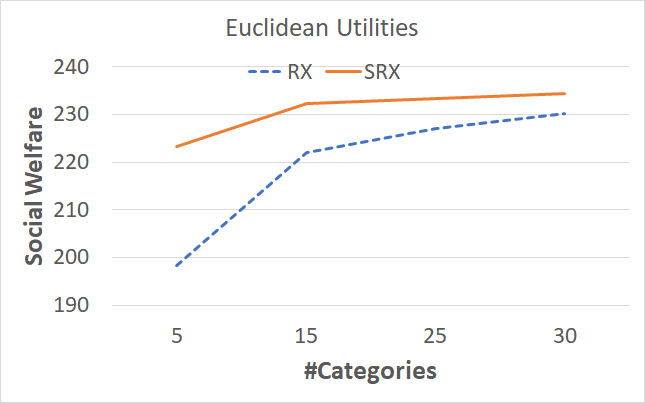
\includegraphics[width=6cm]{simulation/unit_cost_single_sw.png}
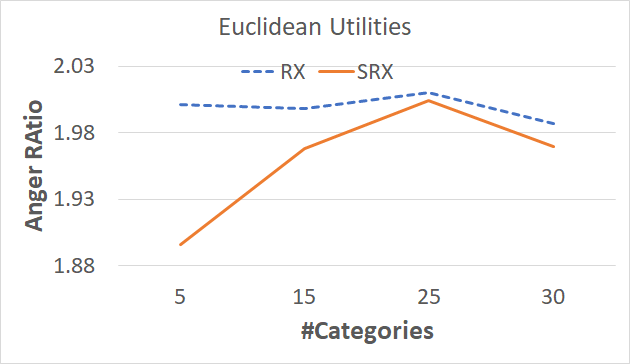
\includegraphics[width=6cm]{simulation/unit_cost_single_ar.png}
\caption{Left: Social welfare  of SRX and RX for different \#categories on Type~1 simulations~ (averaged over 1000 instances) with budget of 20. A higher value is better.\\
 Right: same comparison for the anger ratio. A lower value is better.
}\label{fig:type1}
\end{center}
\end{figure}

\begin{figure}[t]
\begin{center}
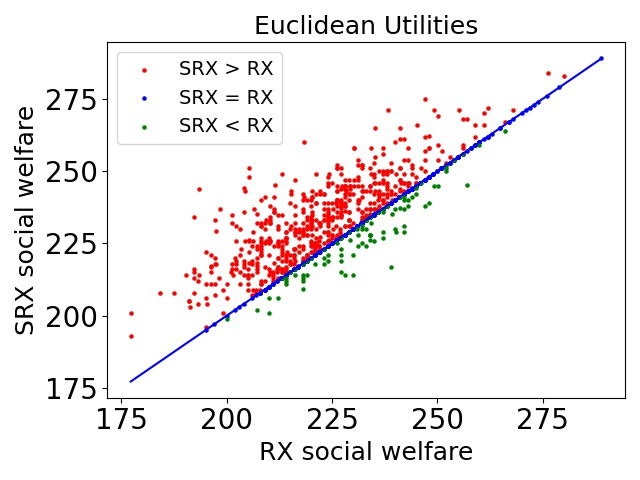
\includegraphics[width=6cm]{simulation/unit_cat(25)_bud(20).jpeg}
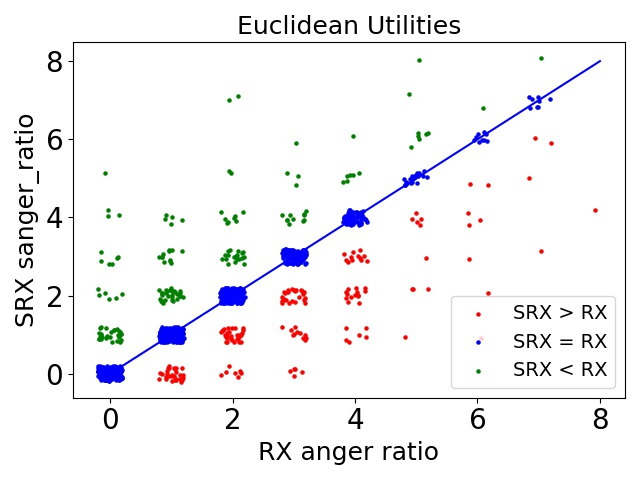
\includegraphics[width=6cm]{simulation/ar_unit_cat(25)_bud(20).jpeg}
\caption{Left: Achieved social welfare by SRX and RX for each of the 1000 instances.\\
Right: Achieved anger ratio by SRX and RX for each of the 1000 instances (with small random value to show point density). Red instances when SRX performs better, green when RX performs better and blue for same value.
% Achieved SW by SRX and RX for each of the 1000 instances (Left for 5 categories and budget of 20 and Right for 25 categories and budget of 20).
 %Top: Social welfare of SRX and RX for different \#approved groups on Type~2 simulations(averaged over 1000 instances). A larger value means a better social welfare.\\
 %Bottom: same comparison for the anger ratio. A smaller value means a better anger.
 }\label{fig:scatter}
\end{center}
\end{figure}

% The  simulation results are  shown in Figures \ref{fig:type1} (for Type~1) and \ref{fig:type2} (for Type~2). 


Figure~\ref{fig:type1} shows how the SW and AR change as the number of categories is increasing (on average). As there are more categories, each voter will have less substitutes in their approved projects. This shows that on average SRX succeeds in achieving higher social welfare compared to RX in all of the scenarios. As the results trend was the same for all budget sizes, the figure shows the results only for budget of 20. Results for all budget sizes can be seen at Appendix~\ref{app:sim}.

As can be seen in the left graph of Figure~\ref{fig:type1}, SRX succeeds to achieve higher social welfare (on average) in all scenarios compared to RX. When looking at the anger ratio in the right graph of the figure, there are more "happy" voters (who get at least one project they wanted) compared to RX. In the constant substitutes scenario (Type~2) the results were similar and can be seen in detail in Appendix~\ref{app:sim}.

% Figure~\ref{fig:type2} shows how the difference in SW and AR changes when letting the voters to approve different number of projects. As the results trend was the same for all cost distributions, the figure show the results only for cost distribution of N(300,20) (results for all budget sizes can be seen at Appendix~\ref{app:sim}).


% As can be seen in the top graphs of both figures, SRX succeeds to achieve higher social welfare (on average) in all scenarios compared to RX. When looking at the anger ratio in the bottom graphs of both figures, in the constant substitutes scenario there are more "happy" voters (who get at least one project they wanted) compared to RX. And in the unit cost scenario,  (bottom of Figure~\ref{fig:type1}) even though SRX satisfies the Strong-BPJR property, compared to RX which satisfies the stronger  EJR property, in most cases voters are more "happy" compared to RX, as determined by the anger ratio. 

One exception is when the budget is limited to 10 (type~1), and RX succeeds in achieving  more happy voters (more details can be seen at Appendix~\ref{app:sim}).

When considering the   simulations in Figure~\ref{fig:type1}, we   see that as the number of categories of projects grow, the closer  the outcomes of RX and SRX become. This result makes sense as  more categories lead to  less  substitute projects and both mechanisms reach similar social welfare and anger ratio. 

Figure~\ref{fig:scatter} present the results for the unit cost scenario from different perspective. This figure shows the achieved social welfare (left) and anger ratio (right) by SRX and RX for each of the 1000 instances, visualising how well each of them did compared to the other and in how many instances. As can be seen in the left plot, SRX succeed in achieving better social welfare in more cases compare to RX ($55\%$ vs $9\%$) Moreover, in the cases where SRX achieve better SW, the difference compare to RX is greater than the other way.

When looking at the right plot, there are about the same amount of cases for each rule which succeed in getting better anger ratio ($16\%$ SRX better and $15\%$ RX better). Actually, in the cases where the budget is 20, for all amount of categories the percentage of instances where each of the rules is better is very close to each other (where SRX have a bit more instances). This result is interesting as, anger ratio give some feeling to how proportional an outcome is, and SRX succeed to compete with RX even through it holds weaker notion of proportionality in this scenario.

While Figure~\ref{fig:scatter} show results only for 25 categories and budget of 20, other scenarios show the same trend. In addition, type~2 scenario achieve even better results (having more instances where both the social welfare and anger ratio of SRX are better). More details about those cases can be seen in Appendix~\ref{app:sim}

% both plots, SRX succeed in achieving better social welfare in more cases compare to RX ($55\%$ vs $9\%$). Moreover, in the cases where SRX achieve better SW, the difference compare to RX is greater than the other way. The results were similar for different \#categories and budgets, as well for the Type~2 scenario. More details about those cases can be seen in Appendix~\ref{app:sim}

% Next, we  look at how the different scenarios affect the outcomes of the SRX mechanism.




% When considering the   simulations in  Figure~\ref{fig:type2}, we   see that as  voters are allowed to approve more projects, the difference in social welfare between SRX and RX increases. This also makes sense, since when voters approve more groups of substitute projects, SRX can achieve better social welfare by splitting the chosen projects between more groups. In contrast, the difference in anger ratio between SRX and RX decreases. In this case, only the voters that want completely different projects from the rest of the population will be hard to satisfy, therefore, there won't much difference between SRX and RX.

 
 One limitation of the simulations is that we chose very specific marginal utility function for substitute projects. If we would have used a different function for all groups or different function for each group, we might have gotten different results. This leads to an interesting question, what is the best way to define the marginal utility functions for each of the substitute groups, which will give the best social welfare and proportionality guarantees.

%%%%%%%%%%%%%%%%%%%%%%%%%%%%%%%%%%%%%%%%%%%%%%%%%%%%%%%%%%%%%%%%%%%%%%%%

\section{Conclusion And Future Work}

In this paper we suggested an input format that allows  voters to express substitute relationships over projects. We extended Rule~X to a modified rule SRX in order to take into account this input format.
We showed that SRX satisfies proportionality in certain scenarios, first it succeed in holding the Extended Justified Representing (EJR) notion of proportionality \cite{peters2020proportional} in constant substitutes scenarios,   and satisfies the  Strong-BPJR \cite{aziz2017proportionally} when having  unit costs for projects without constant substitutes. 

For each of those scenarios we created synthetic simulations which promise to satisfy either EJR or Strong-BPJR. In those simulations SRX succeed to achieve higher social welfare in all scenarios while still being proportional. Moreover, even in cases where SRX holds a weaker notion of proportionality, SRX succeeds in satisfying more voters in the sense that more voters receive at least one project they wants. 

There are several directions we plan for future research:
First is improving the definition of proportionality for the case of substitute projects that will guarantee the voters some utility, rather than number of projects (using the marginal utilities).
Second, while this paper focused on proportionality guarantees for SRX, it is interesting to check what guarantees it possible to get for the social welfare.
Lastly, SRX allows the voters to define any marginal utility they want, however, there might be some family of marginal utility functions which can give better guarantees for both proportionality and social welfare.

%%%%%%%%%%%%%%%%%%%%%%%%%%%%%%%%%%%%%%%%%%%%%%%%%%%%%%%%%%%%%%%%%%%%%%%%
%
% ---- Bibliography ----
%
% BibTeX users should specify bibliography style 'splncs04'.
% References will then be sorted and formatted in the correct style.
%
\bibliographystyle{splncs04nat}
\bibliography{ref.bib}
%

%%%%%%%%%%%%%%%%%%%%%%%%%%%%%%%%%%%%%%%%%%%%%%%%%%%%%%%%%%%%%%%%%%%%%

\clearpage
\begin{subappendices}
\section{Additional Proofs and notes}\label{app:proofs}

Proof for Theorem~\ref{theorem:spr}:
\begin{proof}
Given participatory budgeting scenario E, some $\ell\in \{1,\ldots,L\}$ and $S\subseteq V$  we  assume towards a contradiction that there is some $T\subseteq A$ which all voters in $S$ approve all projects in $T$ and no other project and it holds that $|T\cap R(E)|<|T|$ and $\exists p\in T\setminus R(E), cost(p) +cost(T\cap R(E))\leq \ell$.


We can look at two cases:
\begin{enumerate}
    \item $cost(T)\leq\ell$ - in this case voters $S$ can fund all projects in $T$. Its given that SRX stops with $|T\cap R(E)|<|T|$, but since we know from SRX definition they can't fund projects not from $T$ (as they didn't approved them), it holds that $T\cap R(E)\subset T$. This in that project $p$ still can be funded, in contradiction that SRX stopped.
    
    \item $cost(T)>\ell$ - This mean that group $S$ can't fund all projects in $T$, so it holds that $|T\cap R(E)|<|T|$. From assumption there is some project $p\in T$ such that $cost(p) +cost(T\cap R(E))\leq \ell$ when SRX stops, however, since group $S$ doesn't fund any project outside of $T$, it means that project $p$ can be funded by voters in $S$, in contradiction that SRX stopped
\end{enumerate}
\end{proof}

The requirement that  marginal utilities are non zero is necessary: if in the set of projects $T$ we have substitute projects, funding one of them will make some of the voters not wanting the other items anymore, resulting with only part of $T$ being funded.

However this requirement can sometimes be relaxed. In fact we only require that for any group of voters $S$ such as defined for SPR, their marginal utilities will be defined such they will want (having non zero utility) all projects in $T$. Formally, in addition to requesting that all voter in $S$ approve all projects in $T$ and no other project, we request that $\forall i\in S, \forall g\in v_i, U_{ig}(k)>0 $ for all $k\leq |g\cap T|$.

In addition, in many cases it actually desirable for the marginal utility to be non zero. This is because it can cause cases where there is some project that several voters want it to be funded (some with utility 0 as it is substitute to some funded project), there is enough budget for it, but it won't be funded. While one might claim that it's not funded because the voters don't want a substitute project, it raise the question whether a participatory budgeting mechanism should exhausts its entire budget or leave some of the budget unused.


Proof for Theorem~\ref{theorem:unit}:

\begin{proof}
First, lets notice that at each step SRX have two options to choose a project $p\in A\setminus B_t$, either $p$ not approved by any voter in $S$ or approved by at least one voter $i\in S$.

If $p$ is  not approved by any voter in $S$, it mean that the funds group $S$ have, hasn't changed, so we can ignore this step and look at the next one. If $p$ was approved by some voter $i\in S$, then happen two important things. First, the group $S$ of voter used at most 1 from their total funds in order to fund $p$, this is because all projects are unit cost. Secondly, Since $i\in S$ approved $p$, it means that $|\cup_{i\in S}A_i\cap B_t|$ increased by one.

This mean that in each step, either group $S$ didn't used their funds or they used at most 1 and they got one more approved project. But since group $S$ is T-cohesive, it means that their initial funds are at least $|T|$, this mean that in order to finish their funds they must have funded at least $|T|$ projects, which mean that $|\cup_{i\in S}A_i\cap B_t|\geq |T|$
\end{proof}

\section{Simulation}\label{app:sim}



\begin{figure}[t]
\begin{center}
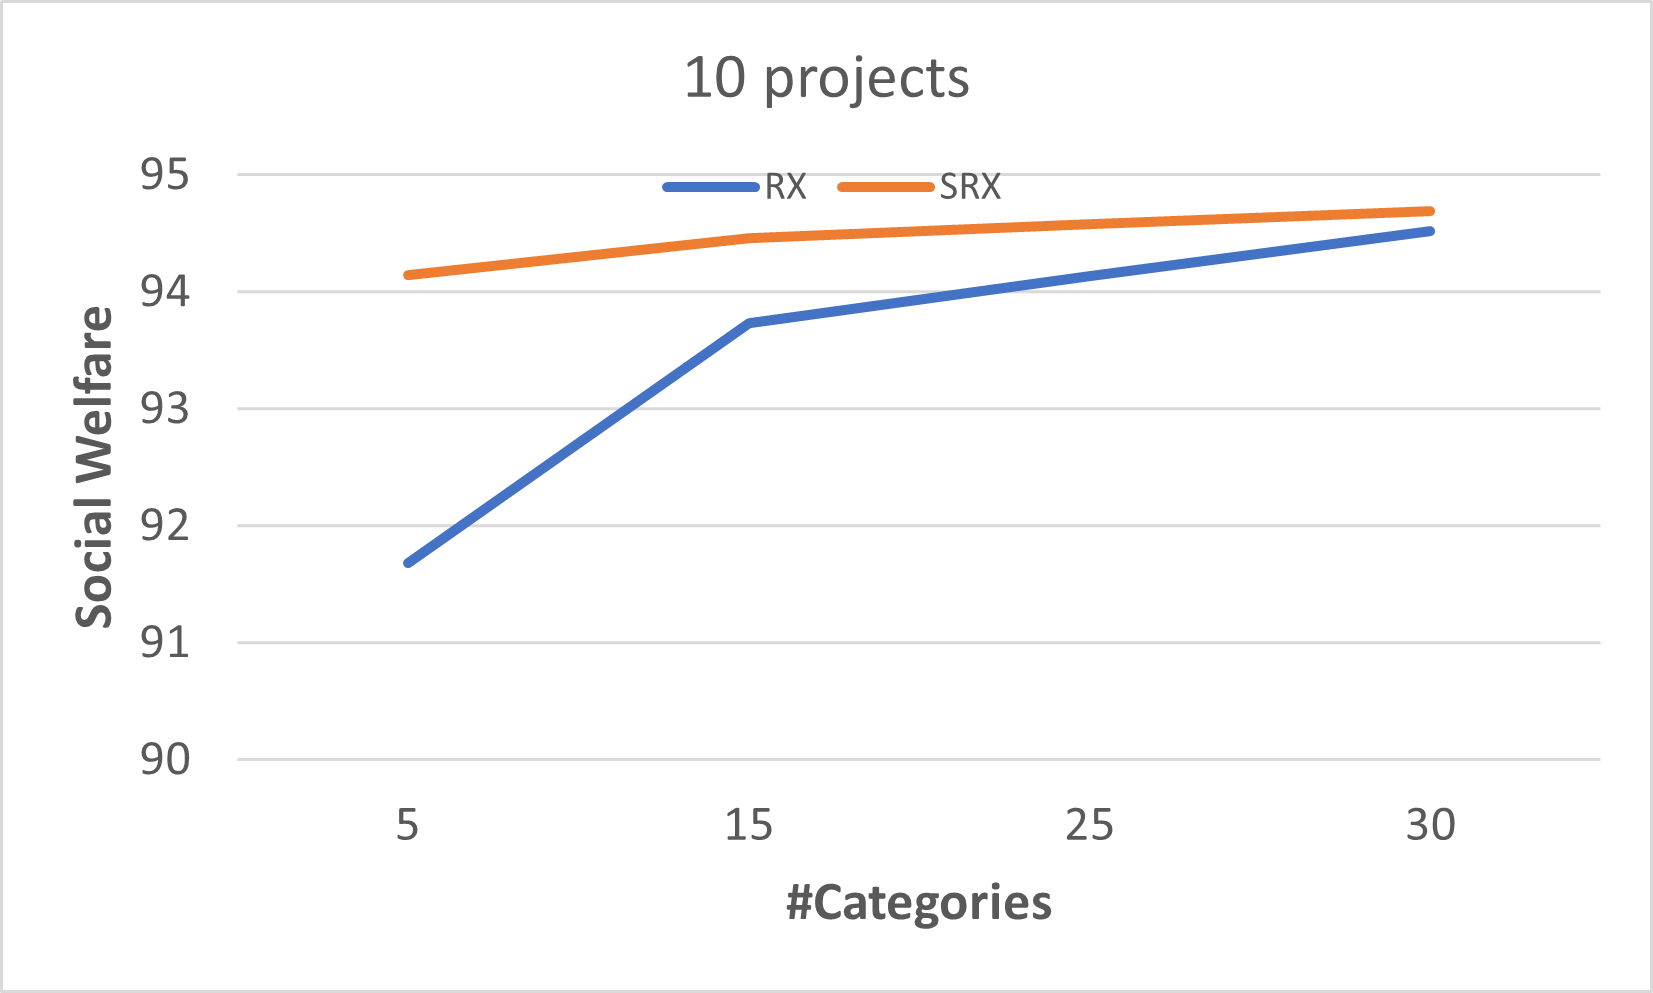
\includegraphics[width=6cm]{simulation/unit_cost_sw_10.png}
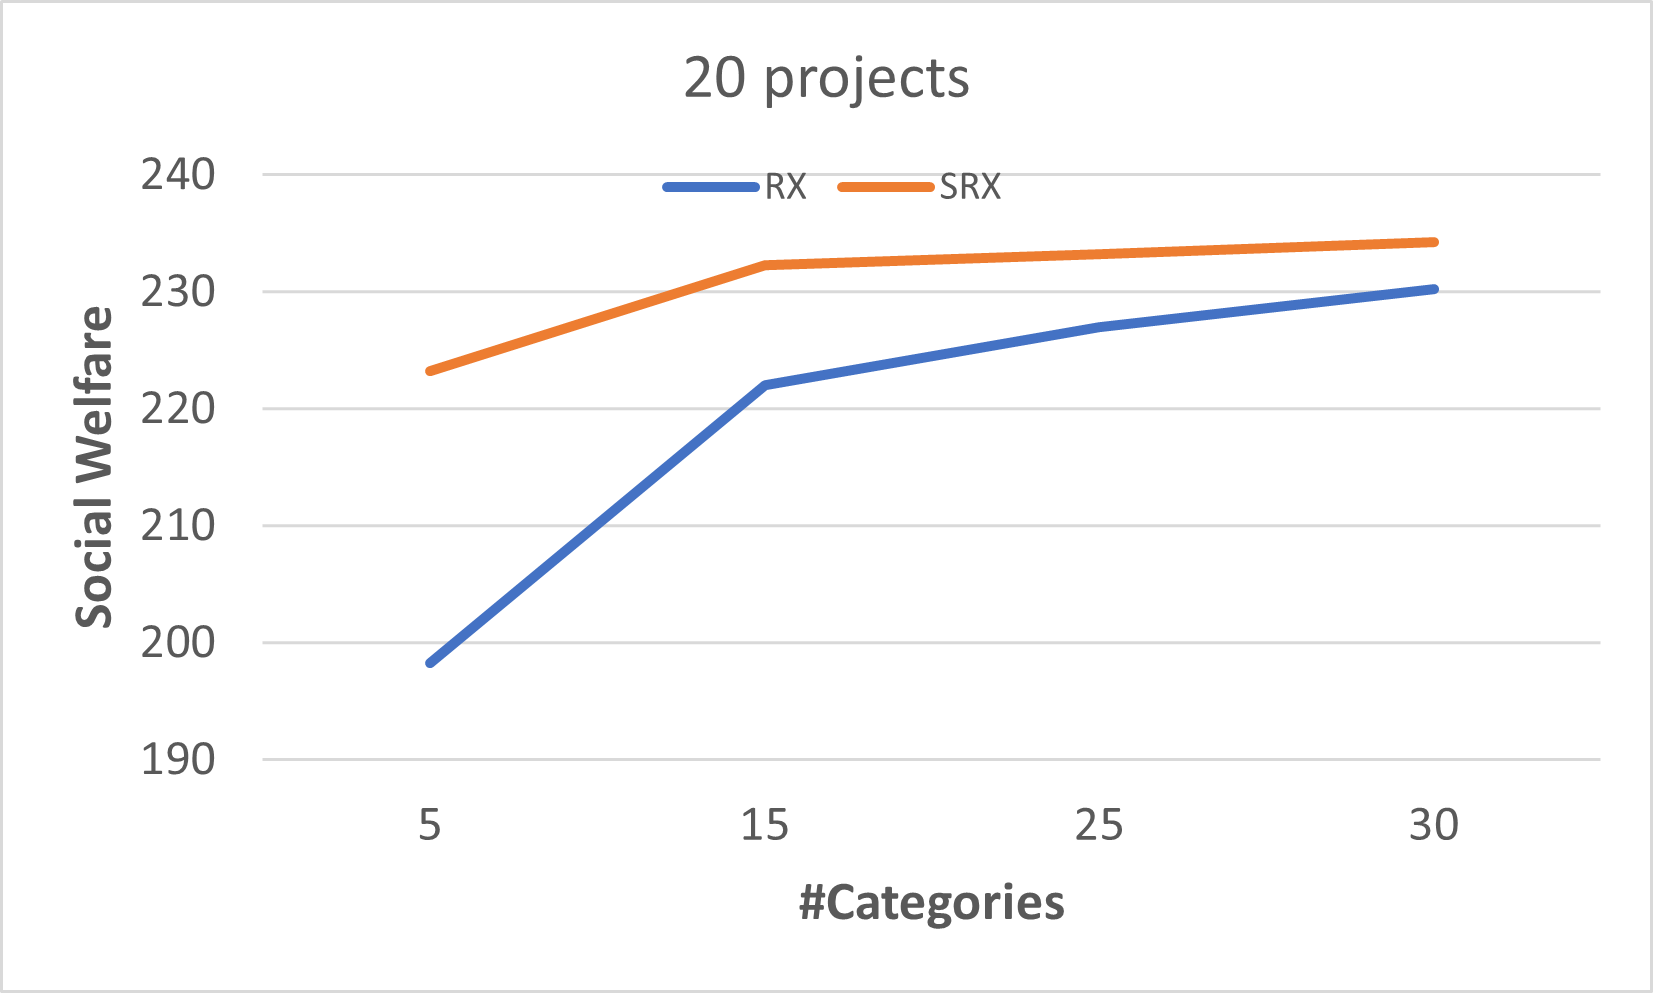
\includegraphics[width=6cm]{simulation/unit_cost_sw_20.png}
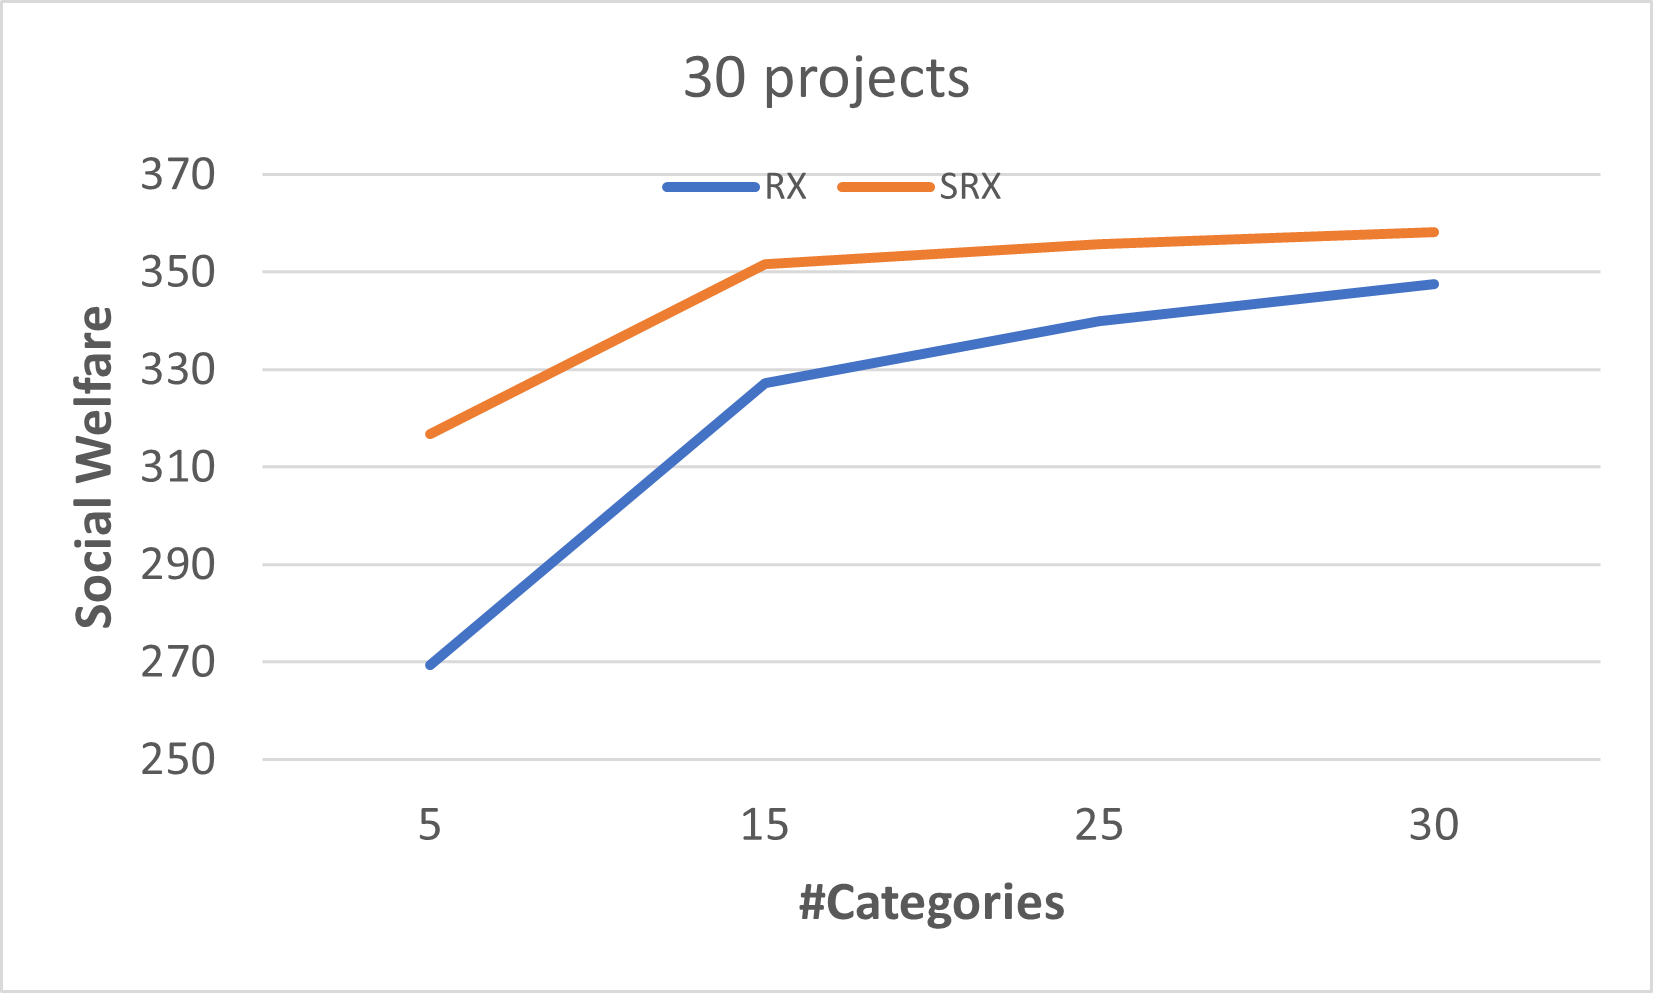
\includegraphics[width=6cm]{simulation/unit_cost_sw_30.png}
\caption{Social welfare achieved by RX and SRX for different size of budget in type~1 scenario.
}\label{fig:sw_all1}
\end{center}
\end{figure}

\begin{figure}[t]
\begin{center}
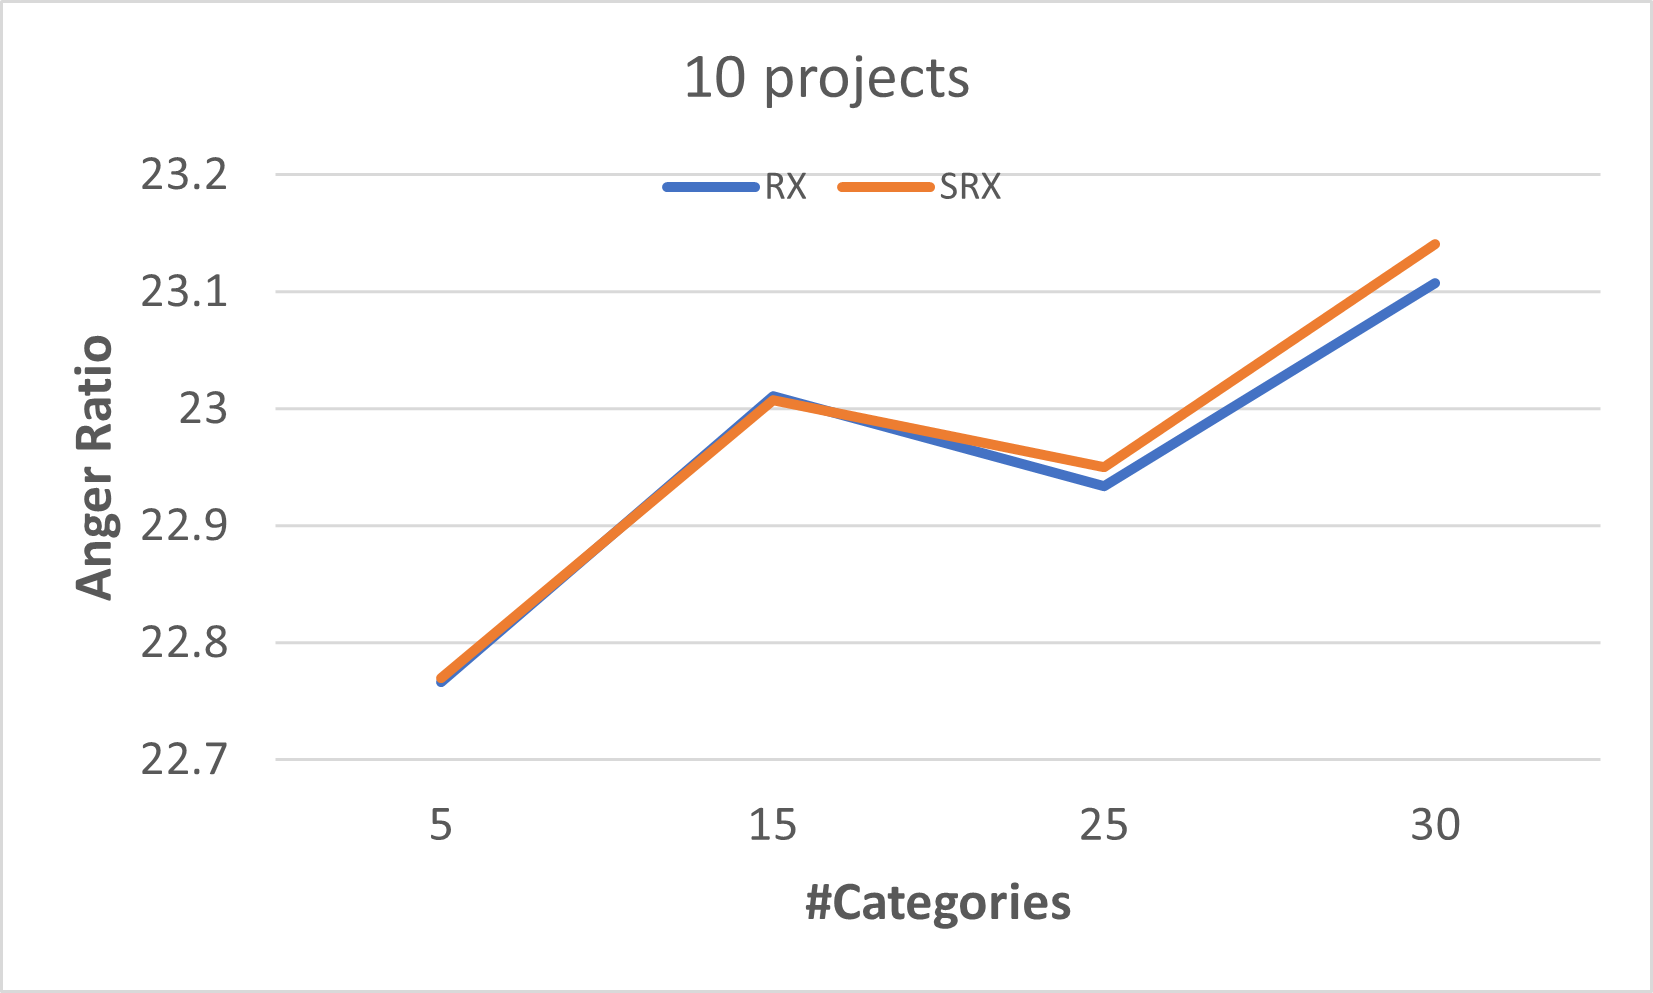
\includegraphics[width=6cm]{simulation/unit_cost_ar_10.png}
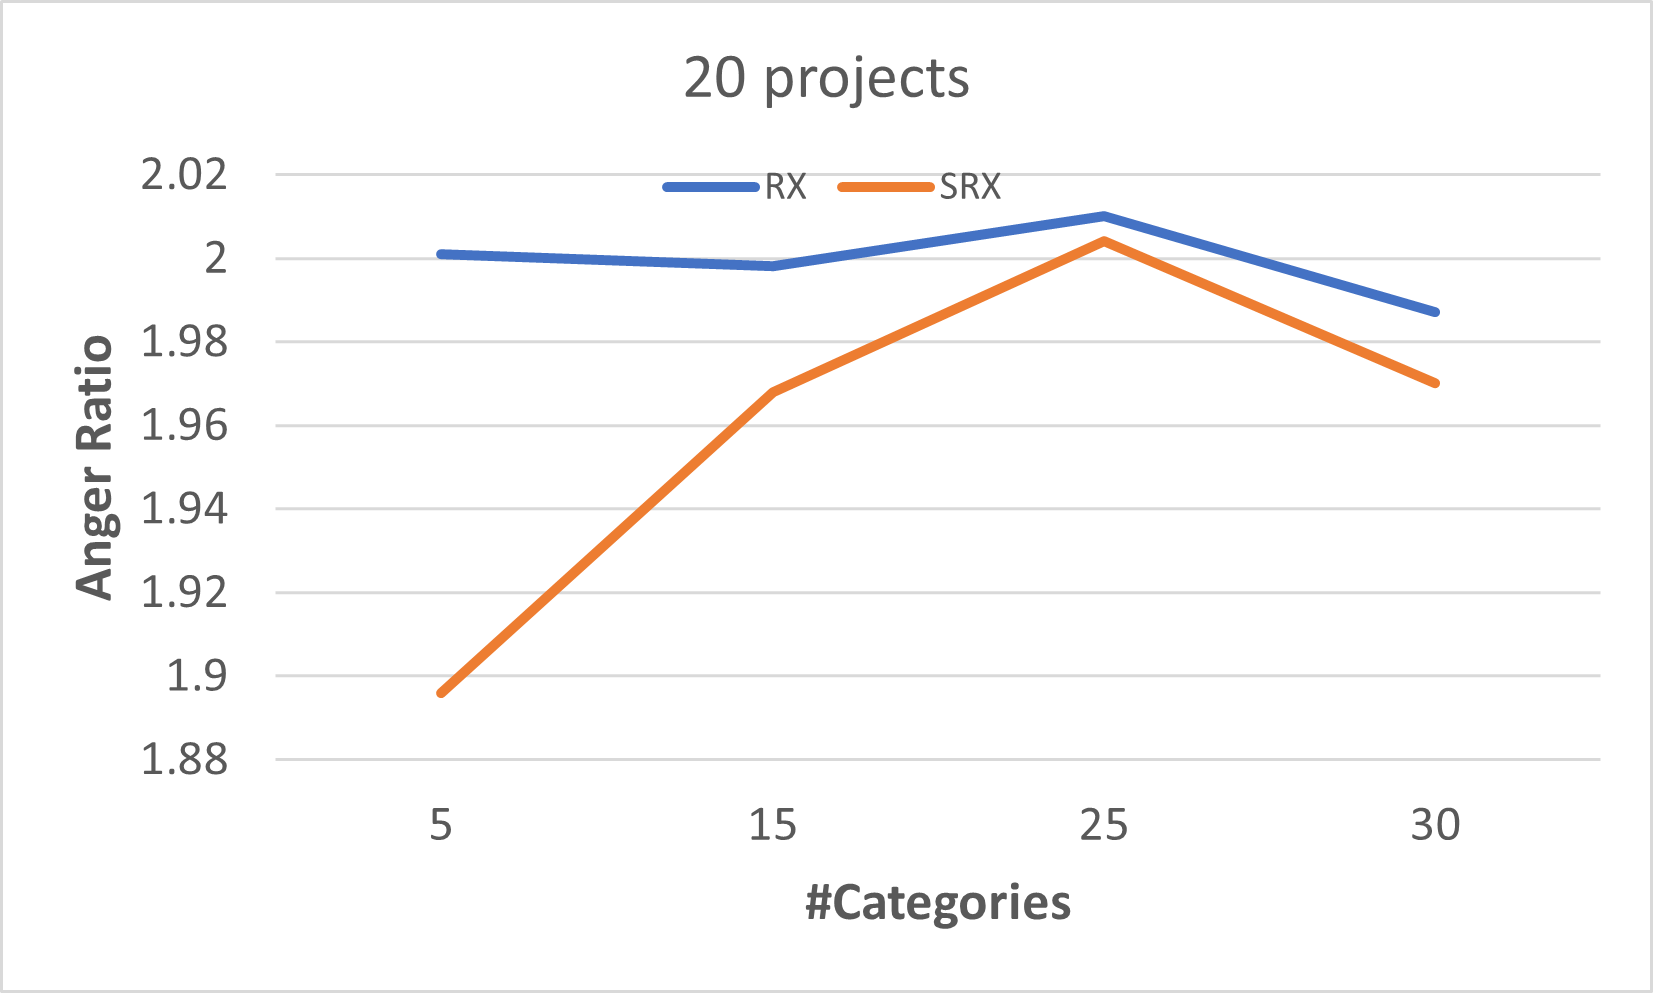
\includegraphics[width=6cm]{simulation/unit_cost_ar_20.png}
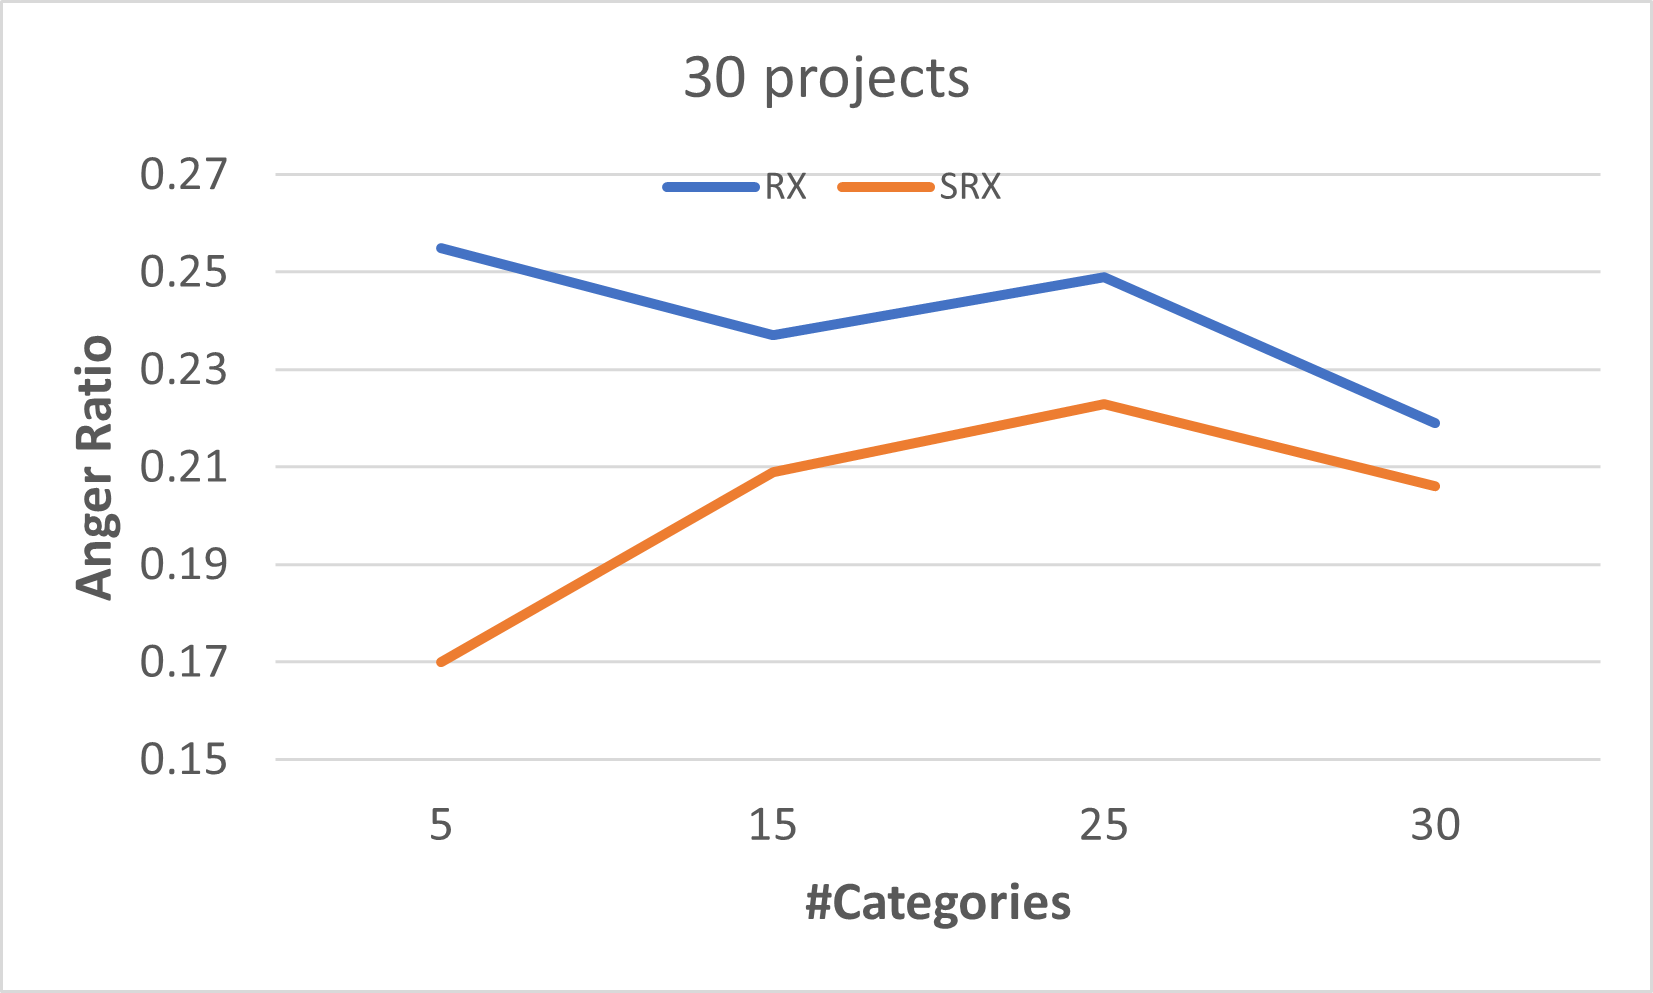
\includegraphics[width=6cm]{simulation/unit_cost_ar_30.png}
\caption{Anger ratio achieved by RX and SRX for different size of budget in type~1 scenario.
}\label{fig:ar_all1}
\end{center}
\end{figure}

% Figure~\ref{fig:type2} shows how the difference in SW and AR changes when letting the voters to approve different number of projects. As the results trend was the same for all cost distributions, the figure show the results only for cost distribution of N(300,20) (results for all budget sizes can be seen at Appendix~\ref{app:sim}).

% When considering the   simulations in  Figure~\ref{fig:type2}, we   see that as  voters are allowed to approve more projects, the difference in social welfare between SRX and RX increases. This also makes sense, since when voters approve more groups of substitute projects, SRX can achieve better social welfare by splitting the chosen projects between more groups. In contrast, the difference in anger ratio between SRX and RX decreases. In this case, only the voters that want completely different projects from the rest of the population will be hard to satisfy, therefore, there won't much difference between SRX and RX.

Figure~\ref{fig:sw_all1} and Figure~\ref{fig:ar_all1} Shows how the size of the project in type~1 simulations affect the social welfare and anger ratio achieved by RX and SRX. As expected the gap between SRX and RX is getting larger as there is a bigger budget, this is because when there is a small budget there isn't a chance to decide between two projects where one of them is substitute to another funded project. Need to say, that in the case where the budget is too small for utilize the advantage of substitutes, RX succeed in achieving better anger ratio (not with big margin).

Figure~\ref{fig:sw_all2} and Figure~\ref{fig:ar_all2} shows how the difference in SW and AR changes when letting the voters to approve different number of projects and using different cost distribution for the projects in type~2 simulations.

When considering those   simulations , we   see that as  voters are allowed to approve more projects, the difference in social welfare between SRX and RX increases. This also makes sense, since when voters approve more groups of substitute projects, SRX can achieve better social welfare by splitting the chosen projects between more groups. In contrast, the difference in anger ratio between SRX and RX decreases. In this case, only the voters that want completely different projects from the rest of the population will be hard to satisfy, therefore, there won't much difference between SRX and RX.


In addition when looking at the effect of different cost distribution, the lower the $\sigma$ chosen for the cost, the higher the difference in voter satisfaction and the lower the difference in anger ratio. This happens because the bigger the $\sigma$ is, there are more cheaper projects, this way it is easier to ignore the the expensive ones and look only the cheap, helping avoid the need to choose between cheap substitute project compared to expensive not substitute project. Lastly, we didn't saw any significant change when using different mean for the cost, therefore, the figure shows only for mean=300.

\begin{figure}[t]
\begin{center}
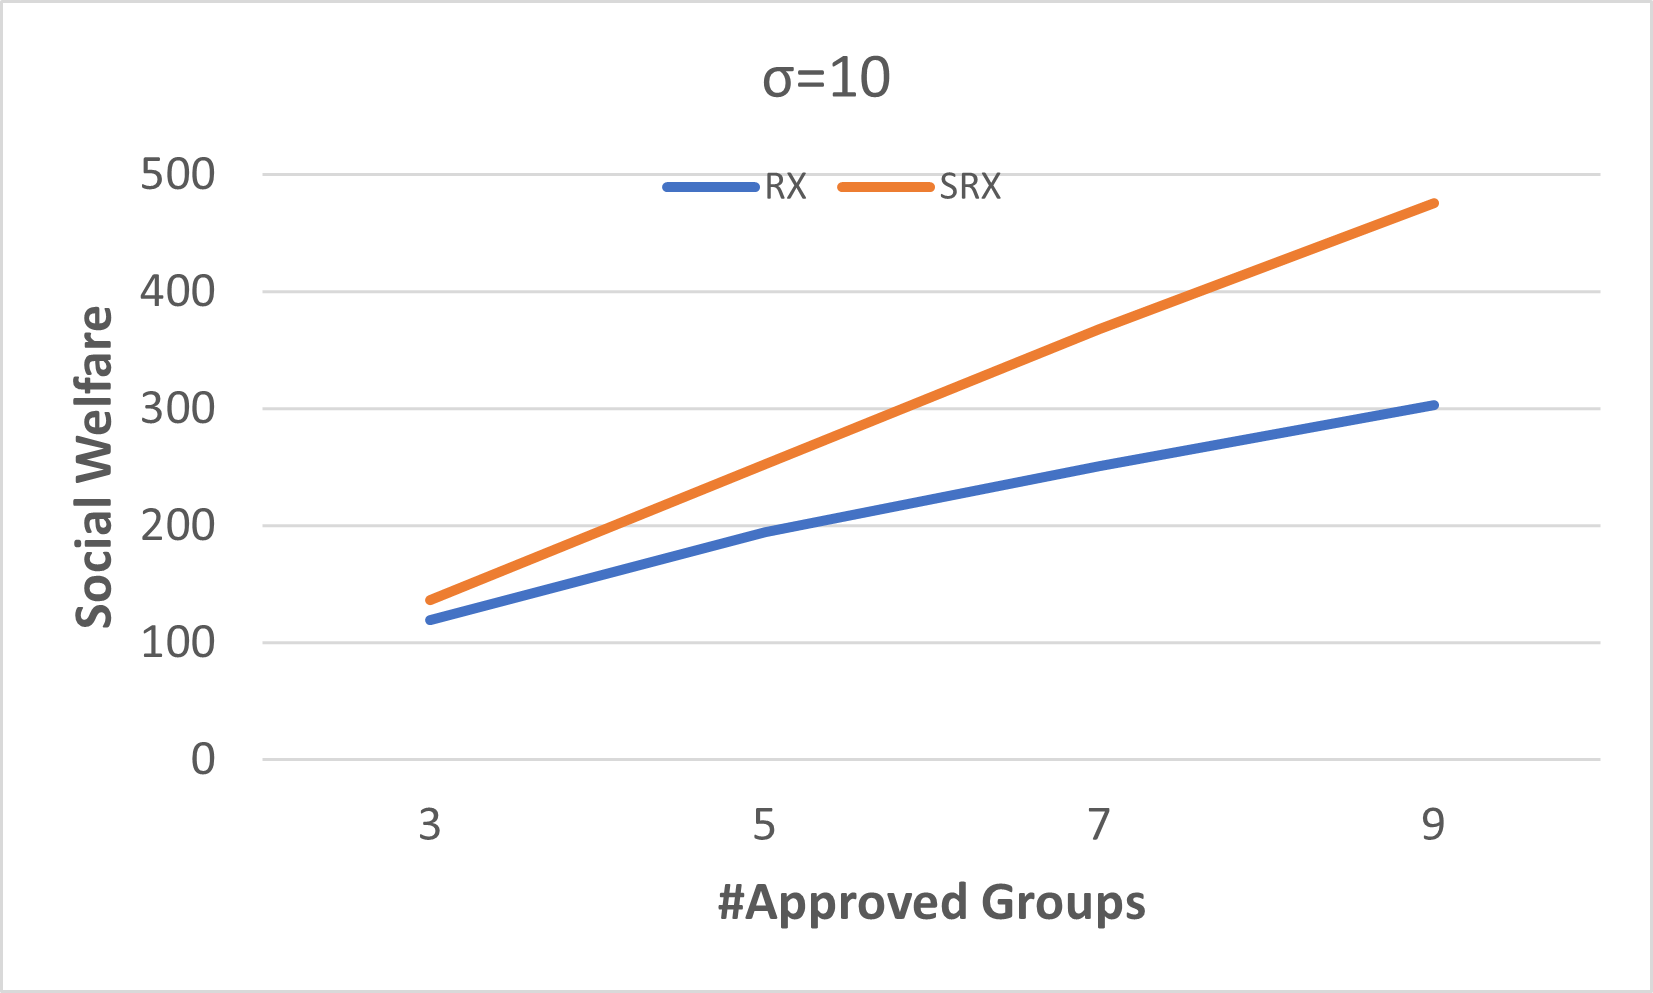
\includegraphics[width=6cm]{simulation/constant_substitutes_sw_10.png}
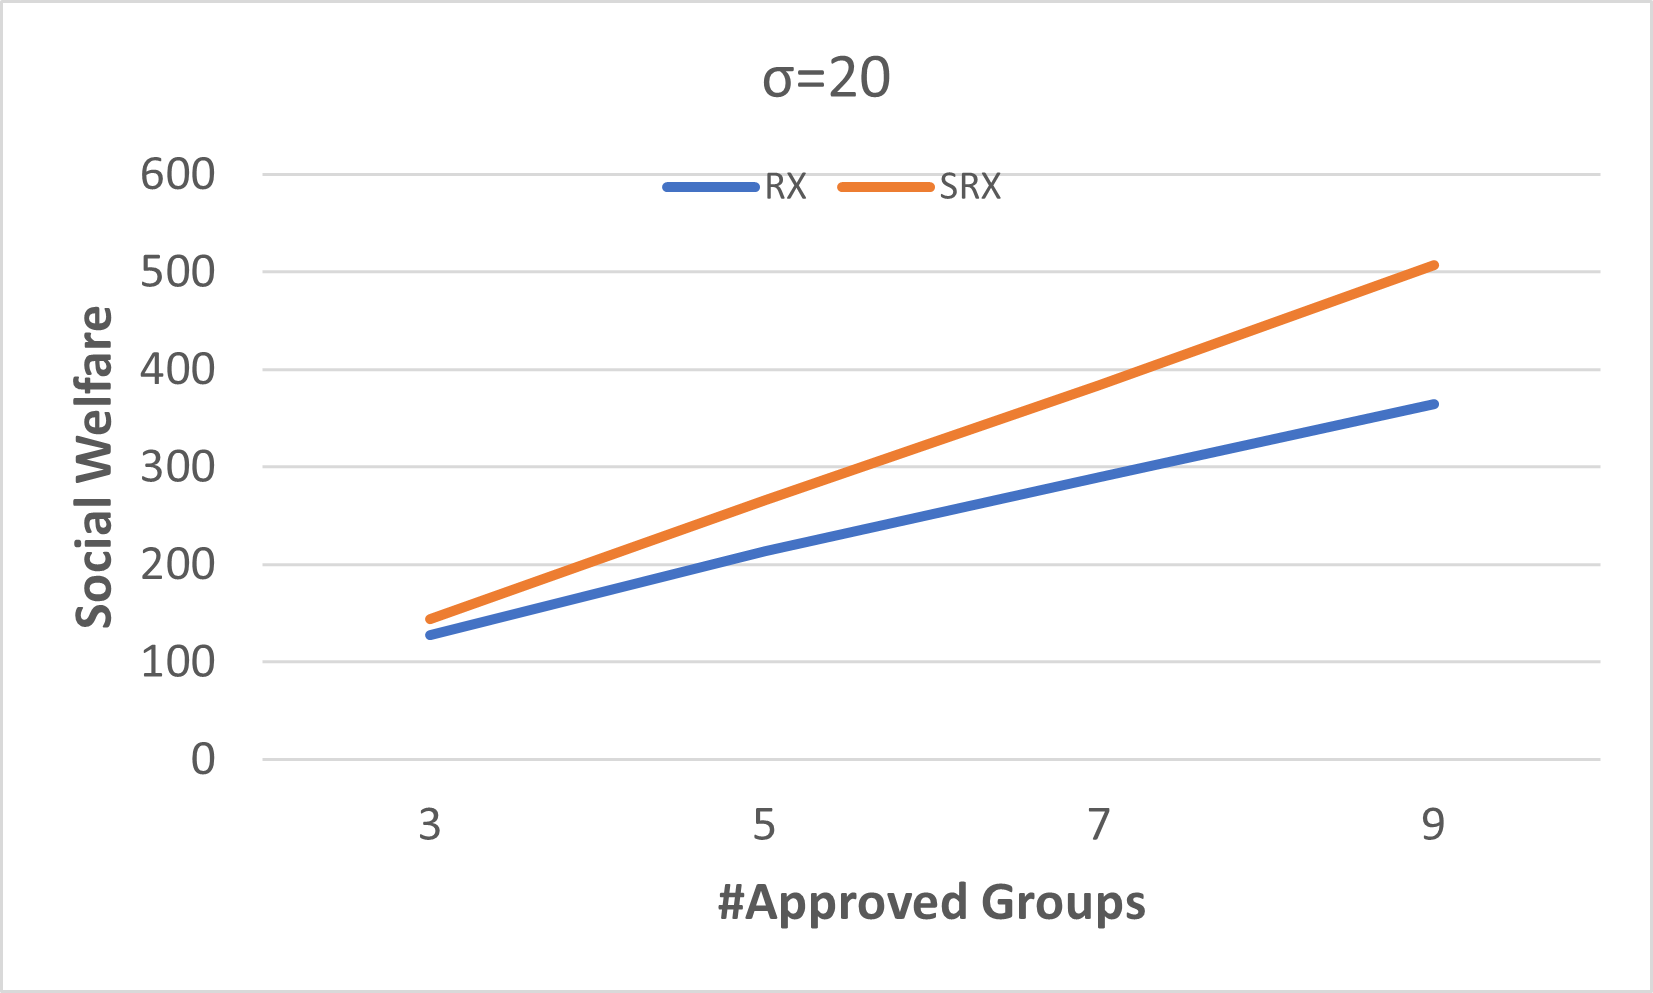
\includegraphics[width=6cm]{simulation/constant_substitutes_sw_20.png}
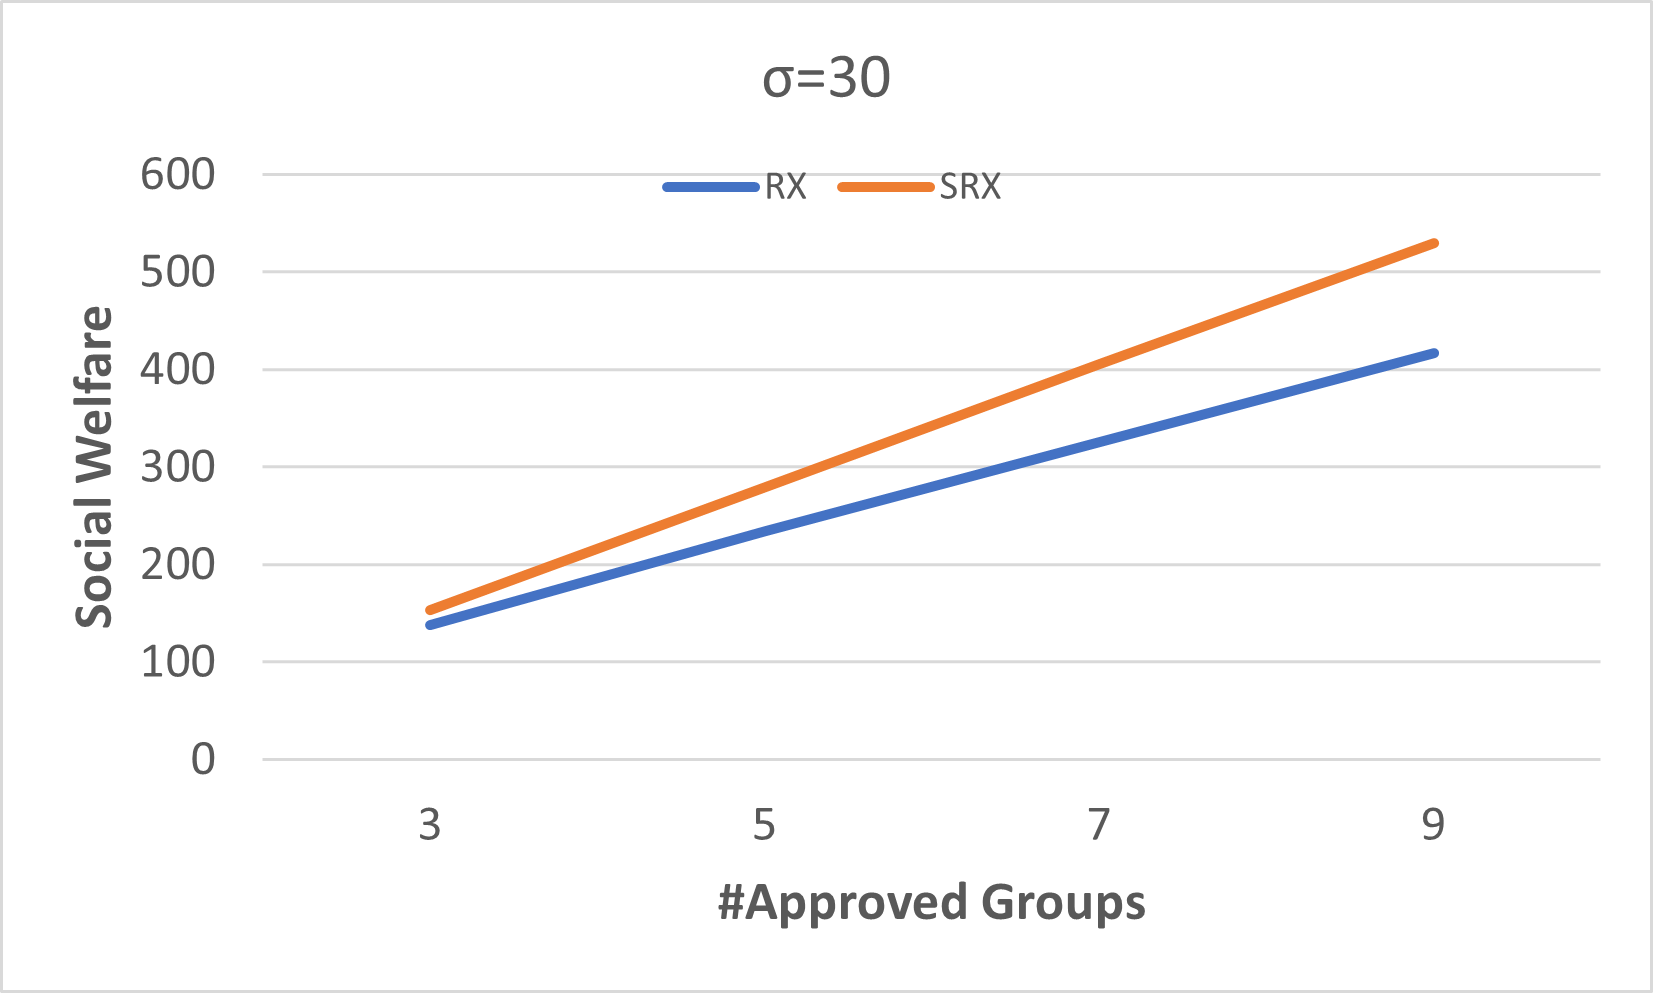
\includegraphics[width=6cm]{simulation/constant_substitutes_sw_30.png}
\caption{Social welfare achieved by RX and SRX for different cost distribution in type~2 scenario.
}\label{fig:sw_all2}
\end{center}
\end{figure}


\begin{figure}[t]
\begin{center}
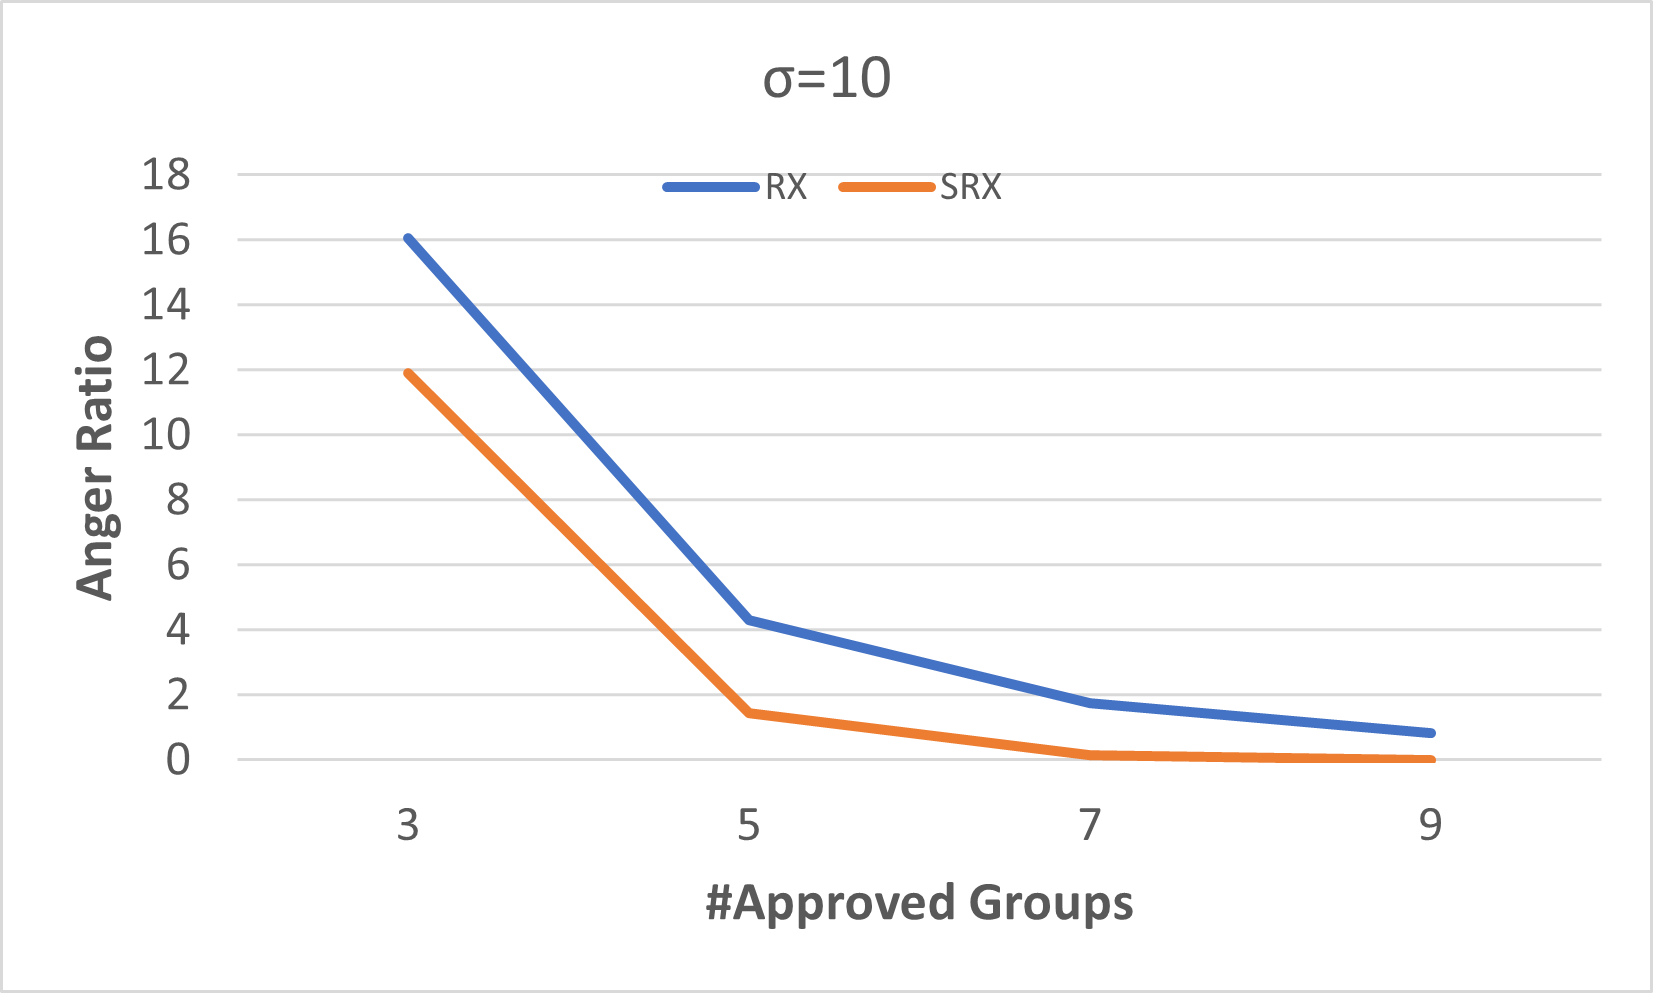
\includegraphics[width=6cm]{simulation/constant_substitutes_ar_10.png}
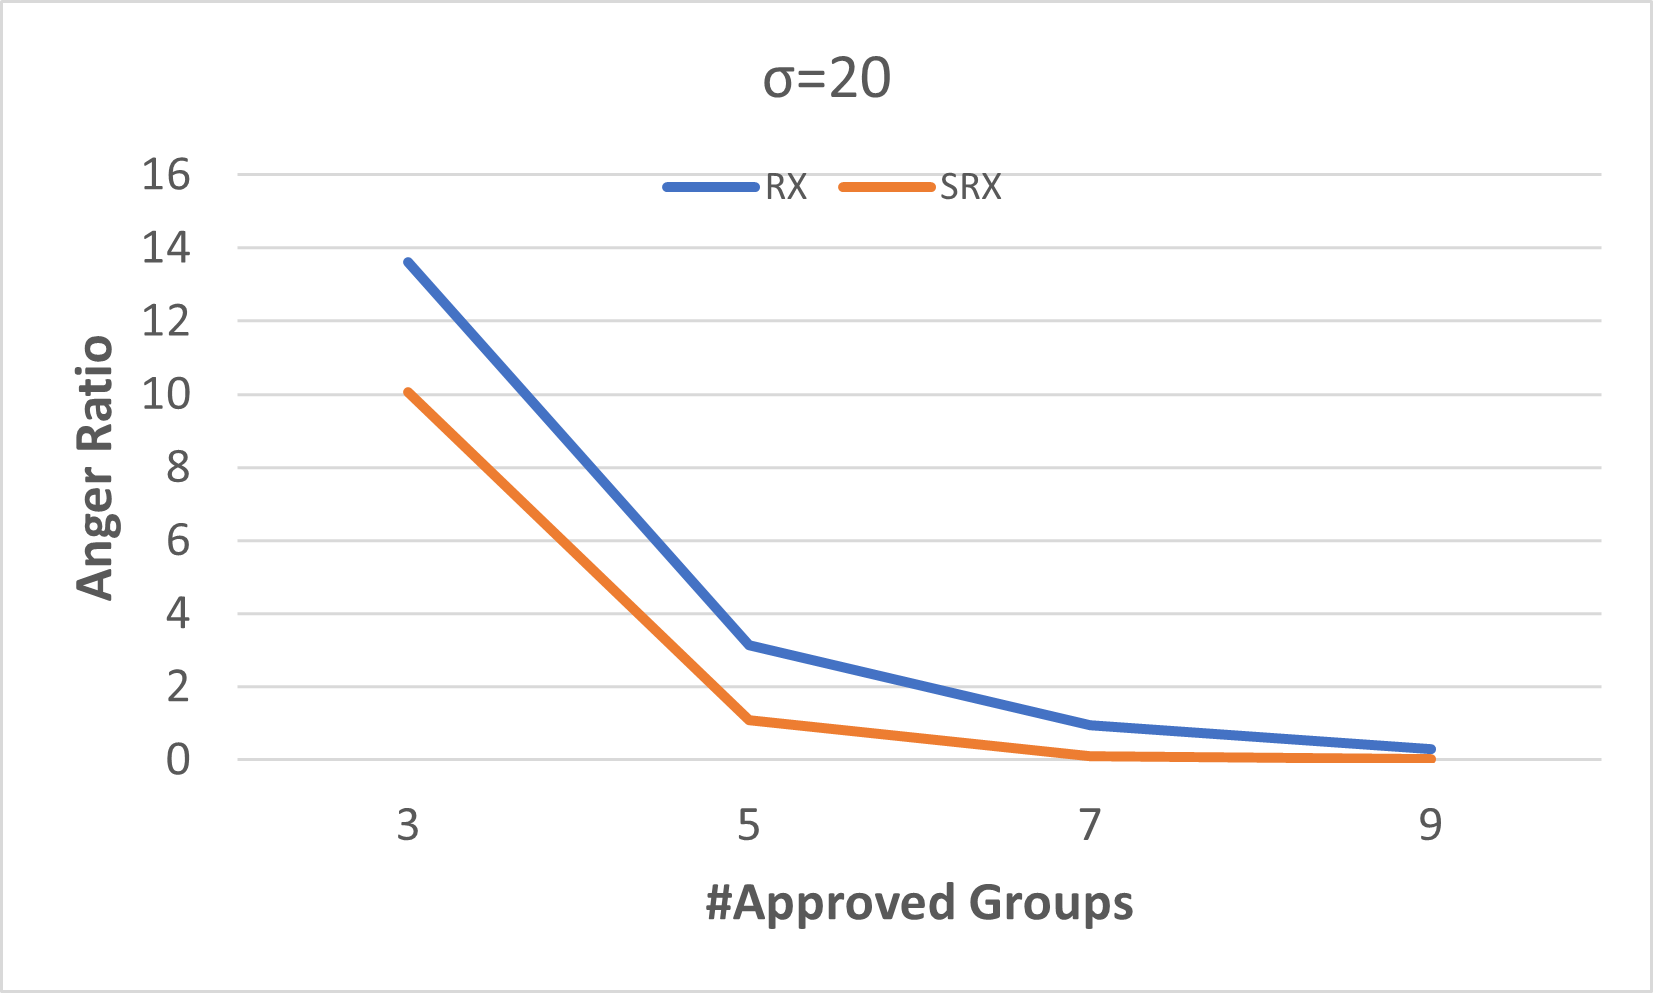
\includegraphics[width=6cm]{simulation/constant_substitutes_ar_20.png}
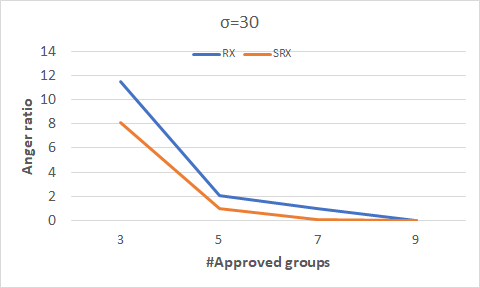
\includegraphics[width=6cm]{simulation/constant_substitutes_ar_30.png}
\caption{Anger ratio achieved by RX and SRX for different cost distribution in type~2 scenario.
}\label{fig:ar_all2}
\end{center}
\end{figure}

Figure~\ref{fig:scatter_all1} and Figure~\ref{fig:scatter_all2} better demonstrates the social welfare SRX and RX succeed achieving in both types of simulations. As mentioned in Section~\ref{sec:exp}, SRX succeed in achieving better social welfare in most instances. In addition the difference in social welfare when SRX is better is bigger than the other way. This is especially notable in Figure~\ref{fig:scatter_all2} where the few instances where RX is better, the difference in SW is pretty much negligible.

When look at the results from the unit cost scenario, it possible to better notice the effect of \#categories and the budget. First, when the budget is small, there isn't a lot of place to "manipulate" the outcome, and in most cases both mechanism result with the same SW. When the budget increase the more power SRX has when considering substitute projects, this is why there are more instances where SRX get better SW than RX when the budget 30 compared to 20.

When looking how the number of categories affect the social welfare, as said in Section~\ref{sec:exp}, SRX are RX are getting closer results as the effect of substitute projects become less meaningful.

Lastly, in Figure~\ref{fig:scatter_all2}, it is possible to see that SRX is better in almost all instances, and even when RX is better, it is by a small difference. This results is especially interesting due the fact that in type~2 simulations, SRX holds EJR in all instances, same as RX. This show that SRX can achieve better outcomes compared to RX without losing level of proportionality in the process.

Figure~\ref{fig:scatter_all_ar1} and Figure~\ref{fig:scatter_all_ar2} better demonstrates the anger ratio SRX and RX succeed achieving in both types of simulations. As mentioned in Section~\ref{sec:exp}, SRX have very close percentage of instances where it achieve better anger ratio to percentage RX achieve.

Looking more closely at Figure~\ref{fig:scatter_all_ar1}, it possible to better notice the effect of \#categories and the budget. Both when the number of categories increase and the budget decrease, SRX and RX are getting more similar anger ratios. This happen because when the number of categories increase, each voter will have less substitutes and the effect of SRX will be more negligible. In addition when having smaller budget, SRX can have less option to "manipulate" the outcome, as it is not enough to fund many substitutes.

Figure~\ref{fig:scatter_all_ar2} demonstrate the disadvantage of to rely on EJR, however, there are cases where this definition is problematic. This is because it possible to hold EJR when a very small amount of voters get several projects they want, while the rest of population doesn't receive any project at all.The measurement of anger ratio present this well as can be seen in the figure. In this scenario, both SRX and RX hold EJR, meaning they both are proportional, however, SRX have much more instances where it every (or less voters compared to RX) voter get at least one project he wanted.

The results from the simulations help to show that SRX compete well against RX. It succeeds in achieving better social welfare, while still satisfying big part of the voters, even in cases where it doesn't hold EJR.


\begin{figure}[t]
\begin{center}
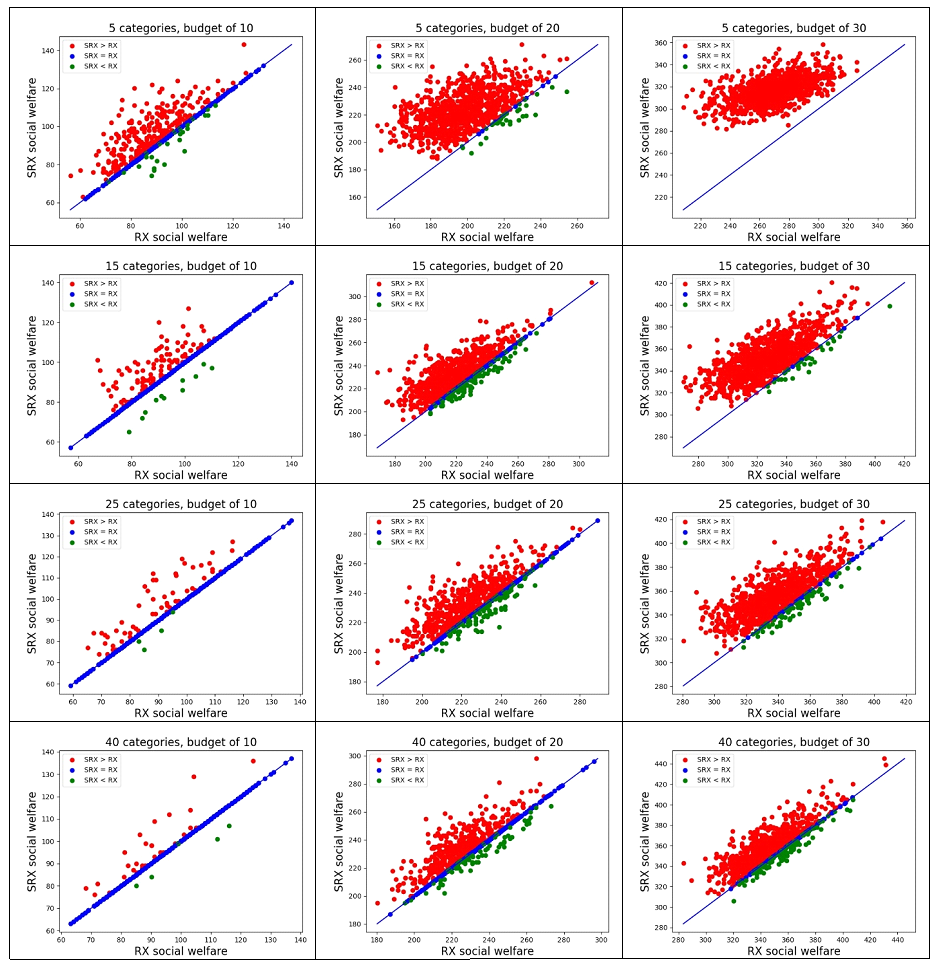
\includegraphics[width=14cm]{simulation/unit_scatters_no_prob.png}
\caption{SRX vs RX social welfare for different instance of type~1 scenario.
}\label{fig:scatter_all1}
\end{center}
\end{figure}

\begin{figure}[t]
\begin{center}
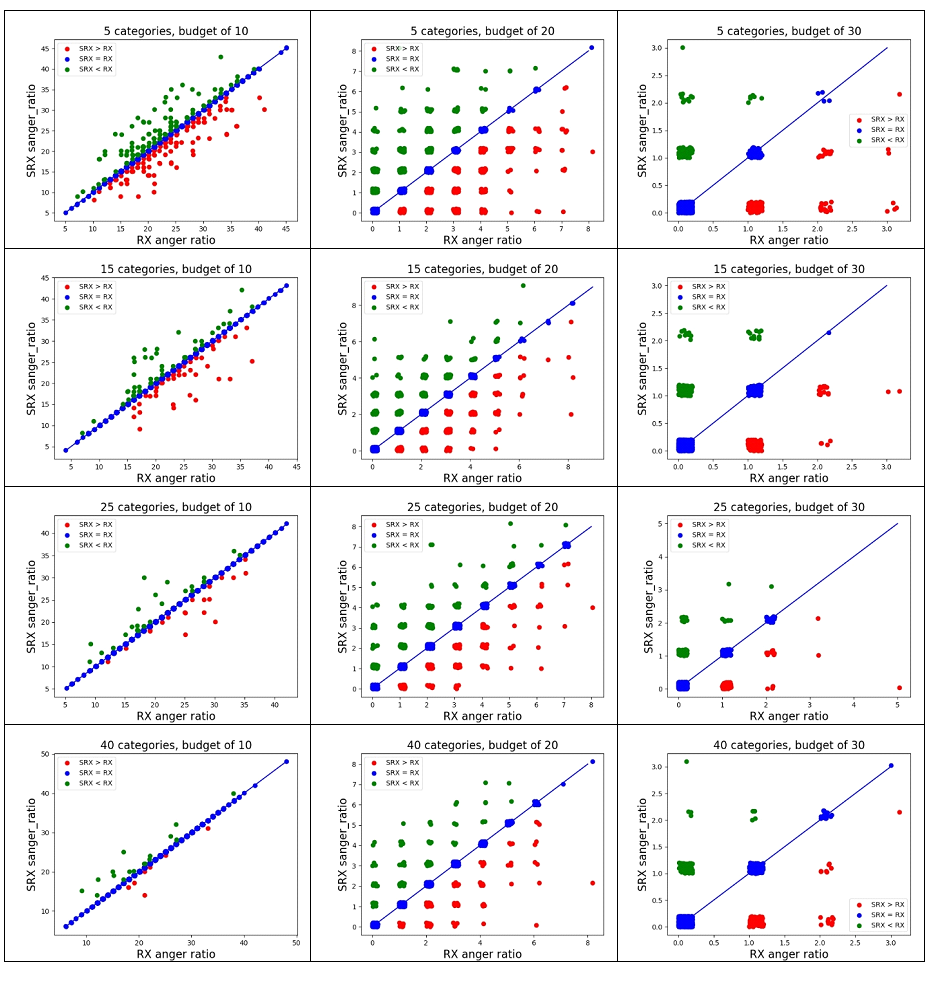
\includegraphics[width=14cm]{simulation/unit_scatters_ar.png}
\caption{SRX vs RX anger ratio for different instance of type~1 scenario.
}\label{fig:scatter_all_ar1}
\end{center}
\end{figure}

\begin{figure}[t]
\begin{center}
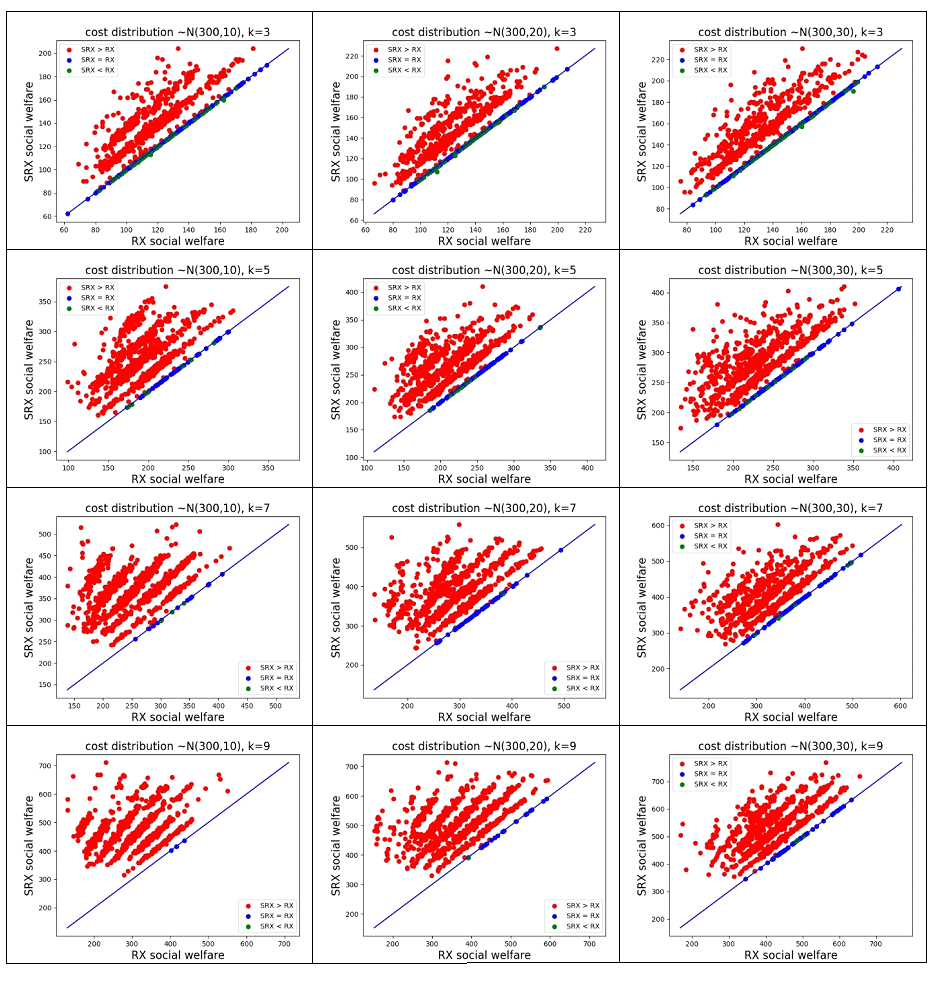
\includegraphics[width=14cm]{simulation/constant_scatters_no_prob.png}
\caption{SRX vs RX social welfare for different instance of type~1 scenario.
}\label{fig:scatter_all2}
\end{center}
\end{figure}

\begin{figure}[t]
\begin{center}
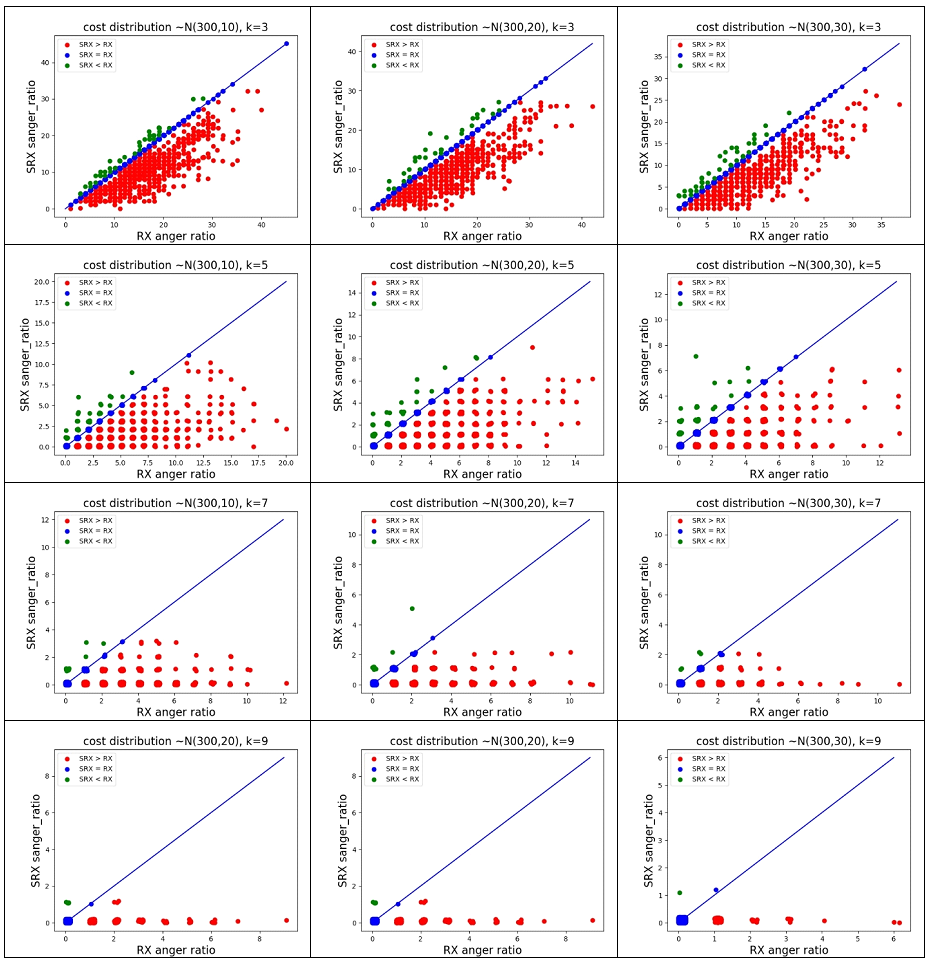
\includegraphics[width=14cm]{simulation/constant_scatters_ar.png}
\caption{SRX vs RX anger ratio for different instance of type~2 scenario.
}\label{fig:scatter_all_ar2}
\end{center}
\end{figure}


\end{subappendices}

\end{document}
